%%
%%  Annexes
%%
%%  Note: Ne pas modifier la ligne ci-dessous. / Do not modify the following line.
\ifthenelse{\equal{\Langue}{english}}{
	\addcontentsline{toc}{compteur}{APPENDICES}
}{
	\addcontentsline{toc}{compteur}{ANNEXES}
}
%%
%%
%%  Toutes les annexes doivent être inclues dans ce document
%%  les unes à la suite des autres.
%%  All annexes must be included in this document one after the other.
\Annexe{Détails des différents domaines de données de l'\ac{API}}\label{ann:api-routes}
\section{API: routes d'appel} 
L'appel routes permet d'énumérer une liste des \ac{URI} disponibles, des méthodes possibles pour chaque \ac{URI} et des fonctions TypeScript appelées par chaque \ac{URI}
\begin{itemize}
    \item GET /api/routes renvoie l'ensemble des routes implémentées sur le serveur. Les colonnes disponibles pour chaque entrée sont listées ci-dessous: 
    \begin{itemize}
        \item path: renvoie l'\ac{URI} pour la route
        \item methods: renvoie une liste des méthodes (GET, PUT, POST, DELETE) pour l'\ac{URI} en question
        \item middlewares: le nom de la fonction TypeScript appelée par le serveur pour renvoyer l'information
    \end{itemize}
\end{itemize}
\section{API: Inventaire} 
Les appels d'API suivants sont proposés pour les objets de type inventaire:
\begin{itemize}
    \item GET /api/inventaire/quartier/$<id_{quartier}>$: Renvoie l'inventaire pour un quartier complet
    \item GET /api/inventaire/calcul/quartier/$<id_{quartier}>$: renvoie le résultat du calcul détaillé dans la section \ref{sec:meth_urb_based_inventory} pour un quartier d'analyse
    \item GET /api/inventaire/calcul/lot/$<g\_no\_lot>$: renvoie le résultat du calcul détaillé dans la section \ref{sec:meth_urb_based_inventory} pour un lot cadastral. Pour l'ensemble des identifiants de lots cadastraux, les espaces dans le numéro de lot sont remplacés par des tirets bas. Ce remplacement est nécessaire pour éviter de mettre des espaces dans l'\ac{URL}.
    \item POST /api/inventaire/calcul/reg-val-man permet de faire un calcul pour des valeurs manuellement entrées par l'utilisateur. Les valeurs manuelles sont transmises dans le corps de la requête. Les entrées suivantes doivent être présentes pour chaque entrée:
    \begin{itemize}
        \item g\_no\_lot: l'identifiant de lot
        \item cubf: le code d'utilisation du bien fond applicable
        \item id\_reg\_stat: l'identifiant de règlement pertinent
        \item id\_er: l'identifiant d'ensemble de règlement pertinent
        \item unite: l'identifiant d'unité de la valeur fournie
        \item valeur: la valeur manuelle entrée par l'utilisateur
    \end{itemize}
    \item POST /api/inventaire/nouv-en-gros: Cette adresse permet de créer des entrées d'inventaire en gros. Les colonnes suivantes doivent être dans le corps de la requête \ac{REST}:
    \begin{itemize}
        \item g\_no\_lot
        \item n\_places\_min
        \item n\_places\_max
        \item n\_places\_mesure
        \item n\_places\_estime
        \item id\_er
        \item id\_reg\_stat
        \item commentaire
        \item methode\_estime
        \item cubf
    \end{itemize}
     \item POST /api/inventaire: nouvelle entrée dans la table \underline{inventaire\_stationnement}. Les informations suivantes sont fournies dans le corps du message:
    \begin{itemize}
        \item g\_no\_lot
        \item n\_places\_min
        \item n\_places\_max
        \item n\_places\_mesure
        \item n\_places\_estime
        \item id\_er
        \item id\_reg\_stat
        \item commentaire
        \item methode\_estime
        \item cubf
    \end{itemize}
    \item PUT /api/inventaire/$<id_{inv}>$: Modification de l'entrée dans la table \ul{inventaire\_ stationnement} dont l'identifiant est égal à la valeur entre <>. Le contenu de l'entrée est communiqué dans le corps du message avec les variables suivantes:
    \begin{itemize}
        \item g\_no\_lot
        \item n\_places\_min
        \item n\_places\_max
        \item n\_places\_mesure
        \item n\_places\_estime
        \item id\_er
        \item id\_reg\_stat
        \item commentaire
        \item methode\_estime
        \item cubf
    \end{itemize}
    \item PUT /api/inventaire/maj-en-gros: permet de faire la modification en gros d'inventaire de stationnement. Contrairement à la mise à jour d'un seul élément, l'ensemble des champs de la table \ul{inventaire\_stationnement} doivent être présents dans le corps de la requête.
   
    
    \item DELETE /api/inventaire/$<id_{inv}>$: supprime l'entrée dont l'id\_inv est égal à la valeur entre <>.
\end{itemize}
\section{API: Règlements}
Les appels d'\ac{API} suivants sont proposés pour les objets de type règlement:
\begin{itemize}
    \item GET /api/reglements/entete: renvoie toutes les entêtes de règlements (description, information administrative). Les paramètres de filtrage suivants peuvent être fournis dans l'\ac{URI} pour réduire la liste de règlements renvoyés. Les éléments description, ville, texte, article et paragraphe utilisent les fonctions de recherches incluses dans PostgreSQL \parencite{postgresql_global_development_group_811_2025}
    \begin{itemize}
        \item annee\_debut\_avant
        \item annee\_debut\_apres
        \item annee\_fin\_avant
        \item annee\_fin\_apres
        \item description
        \item ville
        \item texte
        \item article
        \item paragraphe
    \end{itemize}
    \item GET /api/reglements/complet/<id\_reg\_stat>: renvoie un règlement complet (l'entête et la définition mathématique). Le format JSON renvoyé est le suivant: 
    \begin{itemize}
        \item entete: un vecteur contenant les éléments suivants
        \begin{itemize}
            \item id\_reg\_stat: l'identifiant du règlement
            \item description: description sommaire du règlement
            \item annee\_debut\_reg: Année d'entrée en vigueur du règlement inclusif
            \item annee\_fin\_reg: Année d'abrogation du règlement (inclusif)
            \item texte\_loi: Texte de loi définissant le règlement
            \item article\_loi: Article de loi où le règlement est défini
            \item paragraphe\_loi: Paragraphe de la loi où le règlement est défini
            \item ville: nom commun de la juridiction
        \end{itemize}
        \item définition: une table contenant la définition du règlement avec les éléments suivants
        \begin{itemize}
            \item id\_reg\_stat\_emp: identifiant unique de la ligne de définition mathématique
            \item id\_reg\_stat: identifiant du règlement
            \item ss\_ensemble: sous-ensemble du règlement auquel appartient la ligne
            \item seuil: seuil au dessus duquel le règlement s'applique quand l'opérateur à l'intérieur du sous-ensemble
            \item oper: colonne contenant les opérateur. Le premier élément du sous-ensemble contient l'opérateur applicable entre ce sous ensemble et le précédent, les autres sont l'opérateur utilisé entre les lignes 
            \item cases\_fix\_min: ordonnée à l'origine de la droite représentant le stationnement minimum
            \item pente\_min: pente de la droite représentant le stationnement minimum
            \item cases\_fix\_max: ordonnée à l'origine de la droite représentant le stationnement maximum
            \item pente\_max: pente de la droite représentant le stationnement maximum
            \item unite: unité de l'axes des x de la droite pour les requis minimum et maximum
        \end{itemize}
    \end{itemize}
    \item GET /api/reglements/operations: renvoie le contenu de la table \ul{liste\_operations} (Tableau \ref{tab:operations_table})
    \item GET /api/reglements/unites: renvoie les informations contenues dans la table \ul{multiplicateur\_facteurs\_ colonnes} (Tableau \ref{tab:unite_pertinentes_minimum_stat})
    \item GET /api/reglements/unites/<id>: renvoie la ligne de la table \ul{multiplicateur \_facteurs\_colonnes} dont l'identifiant est entre <>
    \item POST /api/reglements/entete: permet de créer un nouvel entête de règlement. Les éléments suivants doivent être fournis dans le corps du message (voir Tableau \ref{tab:definition_entete_reg_stationnement})
    \begin{itemize}
        \item description
        \item annee\_debut\_reg
        \item annee\_fin\_reg
        \item texte\_loi
        \item article\_loi
        \item paragraphe\_loi
        \item ville
    \end{itemize}
    \item PUT /api/reglements/entete/<id>: permet de modifier un entête de règlement. Les mêmes champs doivent être fournis dans le corps que pour la fonction POST tandis que l'identifiant id\_reg\_stat doit être dans l'adresse.
    \item DELETE /api/reglements/<id>: permet de supprimer le règlement dont l'identifiant id\_reg\_stat est égal à la valeur entre <>
    \item POST /api/reglements/ligne-def: permet de créer une nouvelle entrée dans la table \ul{reg\_stationnement\_empile} (voir Tableau \ref{tab:definition_reg_stat_emp}). Les valeurs suivantes doivent être fournies dans le corps de la requête:
    \begin{itemize}
        \item id\_reg\_stat: identifiant du règlement
        \item ss\_ensemble
        \item seuil
        \item oper
        \item cases\_fix\_min
        \item pente\_min
        \item cases\_fix\_max
        \item pente\_max
        \item unite
    \end{itemize}
    \item PUT /api/reglements/ligne-def/<id>: permet de modifier la ligne de définition mathématique dont l'identifiant (id\_reg\_stat\_emp) est entre <>. Les même champs que la requête POST doivent être fournis.
    \item DELETE /api/reglements/ligne-def/<id>: permet la suppression de la ligne de définition mathématique dont l'identifiant est entre <>.
    \item GET /api/reglements/graphiques: renvoit le nombre de places minimums requises pour le règlement en fonction de l'unité fournie dans les paramètres de requête. Au minimum, les identifiants séparés par des virgules et l'identifiant d'unité doivent être fournis. Les paramètres suivants peuvent être fournis pour raffiner le graphique:
    \begin{itemize}
        \item min: valeur minimale de l'axe des x
        \item max: valeur maximale de l'axe des x
        \item pas: pas pour les valeurs entre min et max
    \end{itemize}
\end{itemize}
\section{API: Ensembles de règlements}
Les appels d'\ac{API} suivants sont proposés pour les ensembles de règlements.
\begin{itemize}
    \item GET /api/ens-reg/entete: renvoie l'ensemble des entêtes de règlements de stationnement dont les propriétés sont listées dans le Tableau \ref{tab:definition_er}:
    \begin{itemize}
        \item id\_er 
        \item date\_debut\_er
        \item date\_fin\_er
        \item description\_er
    \end{itemize}
    \item PUT /api/ens-reg/entete/<id\_er>: permet de modifier l'entête d'ensemble de règlements dont l'identifiant est entre <>. Les paramètres suivants doivent être fournis dans le corps de la requête (voir Tableau \ref{tab:definition_er}):
    \begin{itemize}
        \item description\_er
        \item date\_debut\_er
        \item date\_fin\_er
    \end{itemize}
    \item POST /api/ens-reg/entete/: permet de créer un l'entête d'un nouvel ensemble de règlements. Les mêmes champs doivent être fournis que la fonction PUT.
    \item PUT /api/ens-reg/assoc/<id\_assoc\_er\_reg>: permet de modifier une association spécifique dans un ensemble de règlements. Les champs décrits dans le tableau \ref{tab:definition_association_er_reg_stat}. Les entrées ayant un \ac{CUBF} entre 1 et 9 ne peuvent modifier que le règlement. En effet, au minimum, un ensemble de règlements doit contenir les CUBF 1 à 9. Les variables suivantes doivent être fournies dans le corps de la requête
    \begin{itemize}
        \item id\_reg\_stat, l'identifiant du règlement
        \item cubf, le \ac{CUBF} pour l'utilisation du sol
        \item id\_er, l'identifiant d'ensemble règlement
    \end{itemize}
    \item POST /api/ens-reg/assoc permet de créer une nouvelle association entre un \ac{CUBF} et un règlement. Les variables du tableau \ref{tab:definition_association_er_reg_stat} doivent être fournies:
    \begin{itemize}
        \item id\_reg\_stat, l'identifiant du règlement
        \item cubf, le \ac{CUBF} pour l'utilisation du sol
        \item id\_er, l'identifiant d'ensemble règlement
    \end{itemize}
    \item DELETE /api/ens-reg/assoc/<id\_assoc\_er\_reg> permet de supprimer l'association dont l'identifiant est fourni dans l'\ac{URL}.
    \item GET /api/ens-reg/complet/<id\_er> renvoie  les données suivantes pour l'ensemble de règlement dont l'identifiant est égal à id\_er:
        \begin{itemize}
            \item entete
                \begin{itemize}
                    \item id\_er
                    \item date\_debut\_er
                    \item date\_fin\_er
                    \item description\_er
                \end{itemize}
            \item assoc\_util\_sol
                \begin{itemize}
                    \item id\_assoc\_er\_reg identifiant primaire
                    \item id\_reg\_stat, l'identifiant du règlement
                    \item cubf, le \ac{CUBF} pour l'utilisation du sol
                    \item id\_er, l'identifiant d'ensemble règlement
                \end{itemize}
            \item table\_util\_sol
                \begin{itemize}
                    \item \ac{CUBF}
                    \item description
                \end{itemize}
        \end{itemize}
    \item DELETE /api/ens-reg/<id\_er> permet de supprimer un ensemble de règlements. Le serveur s'assure que cet ensemble n'est pas utilisé dans un ensemble de règlements-territoire avant de supprimer.

\end{itemize}
En plus des adresses basiques fournies ci-dessus, des adresses supplémentaires ont été créées pour certaines pages particulières au sein de l'interface. 
\begin{itemize}
    \item GET /api/ens-reg/reg-associes/<id\_er> renvoie les entêtes des règlements qui sont utilisés dans l'ensemble de règlements dont l'identifiant est égal à id\_er.
    \item GET /api/ens-reg/entete-par-territoire/<id\_periode\_geo> renvoie les entêtes des ensembles de règlements associés au territoire dont l'identifiant est égal à id\_periode\_geo.
    \item GET /api/ens-reg/par-role/<id\_provinc>: permet d'obtenir les entetes d'ensemble de règlements associées à l'inventaire pour une ou plusieurs entrées du rôle. Plusieurs identifiants séparés par des virgules peuvent être fournis entre <>
    \item POST /api/ens-reg/informations-pour-graphique: permet d'obtenir les règlements pertinents et les unités formulées pour les ensembles de règlements et le \ac{CUBF} sélectionné. Les identifiants de règlements et le \ac{CUBF} sont envoyés dans le corps de la requête
\end{itemize}

\section{API: Territoire}
L'\ac{API} possède les appels suivants pour obtenir les territoires. Pour l'instant, aucune fonction n'a été implémenté pour modifier ou supprimer les territoires pour l'instant.
\begin{itemize}
    \item GET /api/territoire/periode/<id\_periode> permet d'obtenir l'ensemble des territoires associés qui sont associés à la période spécifiée dans l'\ac{URL}.
    \item GET /api/territoire/periode-geo/<id\_periode\_geo> permet d'obtenir un territoire selon son identifiant unique.
\end{itemize}
\section{API: Ensembles de règlements territoire}
Les ensemble de règlements territoire sont l'association entre les ensembles de règlements et les territoires. Il s'agit pour l'essentiel d'un assocation entre le territoire et l'ensemble de règlements. Les dates de validités du \ac{RST} sont inférées à partir des dates de validité de l'ensmble de règlement et du territoire. Cet objet a le complément complet d'options pour modifier les associations (contrairement aux territoires et aux quartiers d'analyse qui doivent être téléversés manuellement). Les adresses d'\ac{API} sont les suivants:
\begin{itemize}
    \item GET /api/ens-reg-terr/par-territoire/<id\_periode\_geo>: permet d'obtenir les \ac{RST} associés au territoire dont l'identifiant est spécifié
    \item GET /api/ens-reg-terr/associations: permet d'obtenir des associations en fonction de la latitude, la longitude ou les dates d'entrée en vigueur et d'abrogation au moyen des paramètres de requêtes suivants:
    \begin{itemize}
        \item lat: Latitude en degrés décimal; doit être utilisé avec un longitude
        \item long: Longitude en degrés décimal; doit être utilisé avec une latitude
        \item annee\_debut\_avant: année de début de la période ou de l'ensemble de règlements est avant l'année specifiée
        \item annee\_debut\_apres: année de début de la période ou de l'ensemble de règlements est après l'année spécifiée
        \item annee\_fin\_avant: année de fin de la période ou de l'ensemble de règlements est avant l'année spécifiée
        \item annee\_fin\_apres: année de fin de la préiode ou de l'ensemble de règlements est après l'année spécifiée
        \item ville\_comme: la ville du territoire ressemble à la chaîne de caractères soumise
        \item secteur\_comme: le secteur du territoire ressemble à la chaîne de caractères soumise
    \end{itemize}
    \item POST /api/ens-reg-terr/association: permet de créer une nouvelle association dans la table \underline{association\_er\_territoire} (voir Tableau \ref{tab:definition_association_er_territoire}. Les champs suivants doivent être spécifiés dans le corps de la requête:
    \begin{itemize}
        \item id\_er : l'identifiant du \ac{PRS}
        \item id\_periode\_geo: l'identifiant du territoire
    \end{itemize}
    \item PUT /api/ens-reg-terr/association/<id\_asso\_er\_ter>: permet de modifier l'association dont l'identifiant est entre <>. Les mêmes champs doivent être spécifiés que pour la création d'une nouvelle association
    \item DELETE /api/ens-reg-terr/association/<id\_asso\_er\_ter>: permet de supprimer l'association dont l'identifiant est entre <>.
\end{itemize}
\section{API: Historique}
L'\ac{API}  possède les appels suivants pour manipuler l'historique de la ville:
\begin{itemize}
    \item GET /api/historique obtient l'ensemble des entrées de la table \ul{historique\_geopol} avec les entrées du Tableau \ref{tab:definition_historique_geopol}. Aucun paramètre de filtrage n'a été mis en place à l'heure actuelle pour l'historique du fait de la simplicité des données en cours. 
    \item PUT /api/historique/<$id_{periode}$> permet de modifier un item de la table \ul{historique\_ geopol}. Les colonnes suivantes doivent être dans le corps du message selon les types 
    \begin{itemize}
        \item nom\_periode 
        \item date\_debut\_periode
        \item date\_fin\_periode
    \end{itemize}
    \item POST /api/historique permet de créer une nouvelle période dans la base de données. Les colonnes suivantes doivent être dans le corps du message.
    \begin{itemize}
        \item nom\_periode 
        \item date\_debut\_periode
        \item date\_fin\_periode
    \end{itemize}
    \item DELETE /api/historique/<$id_{periode}$> permet de supprimer la période dont l'identifiant est égal à $id_{periode}$
\end{itemize}


\section{API: Lots cadastraux et entrées du rôle foncier}
Les appels d'\ac{API} suivants ont été implémentés pour les lots cadastraux et les entrées du rôle. Il est important de noter que des fonctions d'association, de création, de mise à jour et de suppression du rôle seraient pertinents pour une implémentation en production. Dans le cadre de ce mémoire, les information du rôle et du cadastre ont été créés manuellement dans la base de données. Finalement, les espaces dans la chaîne de caractères des identifiants doivent être remplacées par le caractère \_.
\begin{itemize}
    \item GET /api/cadastre/lot/quartier-ana/<$id_{quartier}$> permet d'obtenir l'ensemble des lots qui se situent à l'intérieur du quartier d'analyse dont l'identifiant est fourni dans l'\ac{URI}
    \item GET /api/cadastre/lot/<$g\_no\_lot$> permet d'obtenir le lot dont l'identifiant est égal à la valeur fournie de g\_no\_lot.
    \item GET /api/cadastre/role-associe/<$g\_no\_lot$> permet d'obtenir les entrées du rôle foncier associées au lot dont l'identifiant est fourni entre <>. L'identifiant spécifié est celui du lot
\end{itemize}
Une fonction permettant de faire des requêtes complexes en utilisant des boites englobantes est en cours de développement mais incomplète. Elle est principalement pensée pour permettre de réduire le nombre de données géospatiales à garder en mémoire en parcourant la carte. 
\section{API: Codes d'utilisation du Bien-Fonds}
Les appels pour les \ac{CUBF} sont principalement utilisés pour créer les assocations entre les règlements et les utilisations du sol. Pour rendre la recherche plus facile, des paramètres de requête ont été implémentés pour pouvoir obtenir des sous-ensembles pertinents de la liste des \ac{CUBF}. Sans paramètre de requête l'\ac{API} renvoie les 1700 \ac{CUBF}. La création, la modification et la suppression de \ac{CUBF} n'ont pas été implémentés
\begin{itemize}
    \item GET /api/cubf: permet de renvoyer les \ac{CUBF} et leur description. Deux paramètres de requête sont mis en place pour permettre d'extraire des sous-ensembles
    \begin{itemize}
        \item cubf: un \ac{CUBF} numérique. Il est souvent fourni pour chercher les \ac{CUBF} enfants
        \item niveau: donne le niveau du \ac{CUBF}. Un niveau 1 implique un \ac{CUBF} entre 1 et 9, un niveau 2 implique un \ac{CUBF} entre 10 et 99, un niveau 3 implique un \ac{CUBF} entre 100 et 999 et un niveau 4 implique un \ac{CUBF} entre 1000 et 9999
    \end{itemize}
    \item GET /api/n\_entrees: permet de renvoyer le nombre de \ac{CUBF} pour chaque niveau.
\end{itemize}
Quelques exemples seront fournis pour clarifier. L'appel à l'adresse \og{/api/cubf?niveau=1} \fg{} utilisant la méthode GET renvoie les valeurs listées au tableau \ref{tab:get-cubf-niv1}.\par
\begin{table}[h]
    \centering
    \caption{Réponse à l'appel \og{/api/cubf?niveau=1}\fg{}}
    \label{tab:get-cubf-niv1}
    \begin{tabular}{ll}
        \toprule
         CUBF & Description \\
         \midrule
         1 & RÉSIDENTIELLE \\
         2 & INDUSTRIES MANUFACTURIÈRES\\
         3 & INDUSTRIES MANUFACTURIÈRES \\
         4 & TRANSPORTS, COMMUNICATIONS ET SERVICES PUBLICS \\
         5 & COMMERCIALE \\
         6 & SERVICES \\
         7 & CULTURELLE, RÉCRÉATIVE DE LOISIRS \\
         8 & PRODUCTION ET EXTRACTION DE RICHESSES NATURELLES \\
         9 & IMMEUBLES NON EXPLOITÉS ET ÉTENDUES D'EAU\\ \bottomrule
    \end{tabular}
\end{table}
L'appel à la méthode GET à l'adresse \og{/api/cubf?niveau=2\&cubf=6}\fg{} renvoie les entrées au tableau \ref{tab:get-cubf-niv2}\par
\begin{table}[h]
    \centering
    \caption{Réponse à l'appel \og{/api/cubf?niveau=2\&cubf=6}\fg{}}
    \label{tab:get-cubf-niv2}
    \begin{tabular}{ll}
        \toprule
         CUBF & Description \\
         \midrule
         60 & IMMEUBLE À BUREAUX \\
         61 & FINANCE, ASSURANCE ET SERVICE IMMOBILIER\\
         62 & SERVICE PERSONNEL\\
         63 & SERVICE D'AFFAIRES \\
         64 & SERVICE DE RÉPARATION \\
         65 & SERVICE PROFESSIONEL \\
         66 & SERVICE DE CONSTRUCTION \\
         67 & SERVICE GOUVERNEMENTAL\\
         68 & SERVICE ÉDUCATIONNEL\\ 
         69 & SERVICE DIVERS \\\bottomrule
    \end{tabular}
    
\end{table}
L'appel de la méthode GET à l'adresse \og{/api/cubf?niveau=3\&cubf=65}\fg{} renvoie les résultats présentés au tableau \ref{tab:get-cubf-niv3}.\par
\begin{table}[h]
    \centering
    \caption{Réponse à l'appel \og{/api/cubf?niveau=3\&cubf=65}\fg{}}
    \label{tab:get-cubf-niv3}
    \begin{tabular}{ll}
        \toprule
         CUBF & Description \\
         \midrule
         651 & Service médical et de santé \\
         652 & Service juridique\\
         653 & Service Social\\
         654 & Service social hors institution\\
         655 & Service informatique\\
         656 & Service de soins paramédicaux \\
         657 & Service de soins thérapeutiques\\
         659 & Autres services thérapeutiques\\\bottomrule
    \end{tabular}
    
\end{table}
Ainsi, l'inclusion d'un \ac{CUBF} inférieur à 1000 et un niveau approprié permet d'explorer de manière hiérarchique les \ac{CUBF}. Si le niveau n'est pas fourni, seule la description du \ac{CUBF} fourni sera renvoyée.
L'appel à GET \og{/api/cubf/n\_entrees} \fg{} renvoit essentiellement toujours le même résultat donnée au tableau \ref{tab:get-cubf-n-entrees}
\begin{table}[h]
    \centering
    \caption{Réponse de la méthode GET à l'adresse \og{/api/cubf/n\_entrees} \fg{}}
    \label{tab:get-cubf-n-entrees}
    \begin{tabular}{clc}
        \toprule
        Niveau & Description & n\_entrees\\
        \midrule
        1 & CUBF 1 à 9 & 9 \\
        2 & CUBF 10 à 99 & 77\\
        3 & CUBF 100 à 999 & 359 \\
        4 & CUBF 1000 à 9999 & 1255\\
        \bottomrule
    \end{tabular}
    
\end{table}
\section{API: Secteurs d'analyse}
L'\ac{API} permet de manipuler les secteurs municipaux utilisés pour l'analyse qui sont définis à la section \ref{ssec:struct_donnees_sec_analyse}. Les fonctions d'édition et de suppression des quartiers d'analyse n'existent pas à l'heure actuelle. Elles devraient être mise en place dans une version de production de l'outil.
\begin{itemize}
    \item GET /api/quartiers-analyse obtient l'ensemble des quartiers dans la table \ul{sec\_analyse}
\end{itemize}
\section{API: Analyse agrégée}
Plusieurs indicateurs sont agrégés par quartier. Cette section donnera les détails des appels d'\ac{API} permettant de créer les divers graphiques. La ou les variables sélectionnées ainsi que l'ordre de priorité à sélectionner en cas de présence de plusieurs estimés de stationnement sont communiquées au serveur au moyen de paramètre de requête. 3 types d'analyse de quartier sont possibles: cartographique, par diagramme à barre et par diagramme XY. Chaque type d'analyse se voit attribuer un \ac{URI}. Les profils d'accumulation véhicule se voient attribués une \ac{URI} différente de par leur spécificité. D'autre part, les noms de variables doivent être codifiés dans les scripts clients et serveurs tandis que les requêtes SQL ne sont codifiées que dans le script serveur. Une implémentation future devrait permettre de capturer les variables et toutes les informations attenantes dans un seul fichier pour éviter la duplication et de potentielles erreurs. Les codes de variables sont donnés au Tableau \ref{tab:analysis-var-query-vals}.

Les \ac{URI} sont listées ci-dessous:
\begin{itemize}
    \item GET /api/ana-par-quartier/carto: permet d'obtenir une variable pour une carte choroplèthe. Si une variable liée au stationnement est requise, un ordre de priorité des estimés doit être spécifié. Les paramètres de requête sont les suivants:
    \begin{itemize}
        \item variable: identifiant de variable tel que spécifié au tableau \ref{tab:analysis-var-query-vals}
        \item ordre: ordre de priorité. Doit être spécifié comme la suite des chiffres 1 2 et 3 séparés de virgules
    \end{itemize}
    \item GET /api/ana-par-quartier/histo: permet d'obtenir les variables pour un diagramme à barre en fonction du quartier. Si une variable liée au stationnement est requise, un ordre de priorité des estimés doit être spécifié. Les paramètres de requête sont les suivants:
    \begin{itemize}
        \item variable: identifiant de variable tel que spécifié au tableau \ref{tab:analysis-var-query-vals}
        \item ordre: ordre de priorité. Doit être spécifié comme la suite des chiffres 1 2 et 3 séparés de virgules
    \end{itemize}
    \item GET /api/ana-par-quartier/XY: permet d'obtenir les quantités pour un diagramme XY. Les quartiers sont spécifiés dans l'entête de la réponse. Si une variable liée au stationnement est requise, un ordre de priorité des estimés doit être spécifié. Les paramètres de requête sont les suivants:
    \begin{itemize}
        \item X: variable sur l'axe des x
        \item Y: variable sur l'axe des y
        \item ordre: ordre de priorité. Doit être spécifié comme la suite des chiffres 1 2 et 3 séparés de virgules
    \end{itemize}
\end{itemize}
Ainsi, la requête pour obtenir la carte choroplèthe du stationnement total, avec l'ordre de priorité des inventaires étant fixé à \og{Manuel $\rightarrow$ réglementaire manuel $\rightarrow$ Réglementaire automatique} \fg{}  aurait la requête suivante \og{/api/ana-par-quartier/carto?variable=stat-tot\&ordre=1,3,2}\fg{}. Une requête pour les informations d'un graphique XY avec la population en 2021 sur l'axe des X et le stationnement total en axe des y serait \og{/api/ana-par/quartier/XY?X=popu-2021\&Y=stat-tot\&ordre=1,3,2} \fg{}. Les données sont renvoyées de manière à être directement utilisable dans la librairie de graphes de react-chart-js \parencite{ayerst_react-chartjs-2_2017}. Deux adresses supplémentaires sont créées pour recalculer les statistiques agrégées
\begin{itemize}
    \item GET /api/ana-par-quartier/recalcule-stat-agreg: permet de recalculer le nombre de places de stationnement pour chaque quartier
    \item GET /api/ana-par-quartier/recalcule-val-autres: permet de recalculer les statistiques issues de l'enquête OD, du recensement ou du rôle foncier pour chaque quartier
\end{itemize}
\section{API: Profiles d'accumulation véhicule}
Les appels d'\ac{API} suivants sont mis en place pour gérer les profils d'accumulation véhicule \parencite{diallo_methodology_2015,morency_characterizing_2008} qui permettent de trouver la \og{population}\fg{} de véhicules dans une géographie en fonction de l'heure de la journée.
\begin{itemize}
    \item GET /api/PAV?order=<X,Y,Z>\&id\_quartier=<$id_{quartier}$> permet d'accéder au profile d'accumulation véhicule pour le quartier dont l'identifiant est spécifié. L'ordre spécifié donne l'ordre de préséance pour le relevé de l'inventaire du quartier. En effet, l'\ac{API} fournit l'inventaire du quartier en même temps pour visuellement constater l'utilisation de la capacité. Les données sont fournies de manière à être utilisées par react-chart-js \parencite{ayerst_react-chartjs-2_2017}.
    \item GET /api/PAV/recalcule/<$id_{quartier}$> permet de refaire le calcul du profile d'accumulation véhicule à partir des données de l'enquête OD
    \item POST /api/PAV/<$id_{quartier}$> permet de mettre à jour le profile d'accumulation dans la base de données une fois que l'utilisateur l'a confirmé
\end{itemize}
\section{API: Validation}
L'\ac{API} de validation a été mis en place pour permettre de rapidement assurer la qualité de l'inventaire créé. Bien que des développements méthodologiques demeurent, l'implémentation actuelle a les fonctionnalités de base pour créer une structure d'échantillonnage stratifiée, de sélectionner un ensemble de lots selon la méthodologie choisie, d'entrer les données de validation et de visualiser les résultats. Cette section documentera les appels d'\ac{API} mise en place pour soutenir cette fonctionnalité  
\clearpage

\Annexe{Détails des données de réglementaires}
\section{Ensembles de règlements créés}\label{sec:annex-prs-created}
Le tableau suivant donne une liste des ensembles de règlements créés:
\begin{longtable}{p{10cm}cc}
\caption{Liste des ensembles de règlements crées} \label{tab:liste-er-crees} \\
\toprule
Description & Année début & Année Fin \\
\midrule
\endfirsthead
\multicolumn{3}{c}%
{{\tablename  ~\thetable{} -- suite de la page précédente}} \\[0.5ex] \\
\midrule
Description & Année début & Année Fin \\
\midrule
\endhead
\midrule
\multicolumn{3}{r}{Continué à la page suivante} \\
\midrule
\endfoot
\bottomrule
\endlastfoot
Lac St-Charles - Remplissage & Perpétuité & 1987 \\
Sillery - Remplissage & Perpétuité & 1994 \\
St-Émile - Remplissage & Perpétuité & 1989 \\
Ste-Foy - Remplissage & Perpétuité & 1994 \\
Val-Belair - Remplissage & Perpétuité & 1987 \\
Vanier - Remplissage & Perpétuité & 1992 \\
Lorretteville - Remplissage & Perpétuité & 1994 \\
CUQ - HV-BV-Limoilou - Général - Placeholder & Perpétuité & 1994 \\
CUQ - Des Rivières - Placeholder & Perpétuité & 1994 \\
Beauport - Remplissage & Perpétuité & 1986 \\
Cap Rouge - Remplissage & Perpétuité & 1994 \\
Charlesbourg - Remplissage & Perpétuité & 1995 \\
Beauport - 87-806 & 1987 & 2009 \\
Lac St-Charles - 88-257 & 1988 & 2009 \\
Val-Belair - VB-344-88 & 1988 & 2009 \\
St-Émile - 310-89 & 1989 & 2009 \\
Vanier - 93-05-1245 & 1993 & 2009 \\
CUQ - Des Rivières & 1995 & 2009 \\
Cap-Rouge - 1151-95 & 1995 & 2009 \\
Ste-Foy - 3501 & 1995 & 2009 \\
Sillery - 950 & 1995 & 2009 \\
CUQ - HV-BV-Limoilou - Prioritraire & 1995 & 1996 \\
CUQ - HV-BV-Limoilou - Général & 1995 & 1996 \\
Lorretteville -1386 & 1995 & 2009 \\
Charlesbourg - 96-2921 & 1996 & 2009 \\
CUQ - Abrogation secteur prioritaire - VQ - HV & 1997 & 2009 \\
CUQ - Abrogation secteur prioritaire - Maizerets & 1997 & 2009 \\
CUQ - Abrogation secteur prioritaire - St-Jean-Baptiste & 1997 & 2009 \\
CUQ - Abrogation secteur prioritaire - Montcalm & 1997 & 2009 \\
CUQ - Abrogation secteur prioritaire - st-sacrement & 1997 & 2009 \\
CUQ - Abrogation secteur prioritaire - Lairet & 1997 & 2009 \\
CUQ - Abrogation secteur prioritaire - Vieux-Limoilou & 1997 & 2009 \\
CUQ - Abrogation secteur prioritaire - Saint Roch & 1997 & 2009 \\
CUQ - Abrogation secteur prioritaire - St-Sauveur & 1997 & 2009 \\
CUQ - Abrogation secteur prioritaire - Cap-Blanc & 1997 & 2009 \\
CUQ - Abrogation secteur prioritaire - VQ - BV & 1997 & 2009 \\
Québec - post harm - structurant B & 2010 & 2015 \\
Québec - post harm - général & 2010 & 2015 \\
Québec - post harm - structurant A & 2010 & 2015 \\
Québec - post harm - urbain dense & 2010 & 2015 \\
Québec - Refonte hotellerie - structurant A & 2016 & 2018 \\
Québec - Refonte hotellerie - général & 2016 & 2018 \\
Québec - Refonte hotellerie - structurant B & 2016 & 2018 \\
Québec - Refonte hotellerie - urbain dense 2016 & 2016 & 2017 \\
Québec - modification alimentaire - urbain dense & 2018 & 2018 \\
Québec - modification poste de carburant et minigolf - structurant B & 2019 & 2019 \\
Québec - modification poste de carburant et minigolf - structurant A & 2019 & 2019 \\
Québec - modification poste de carburant et minigolf - urbain dense & 2019 & 2019 \\
ER ITE dummy & 2019 & 2023 \\
Québec - modification poste de carburant et minigolf - général & 2019 & 2019 \\
Québec - refonte hotelliere 2 - général & 2020 & 2023 \\
Québec - refonte hotelliere 2 - urbain dense & 2020 & 2023 \\
Québec - refonte hotelliere 2 - structurant A & 2020 & 2023 \\
Québec - refonte hotelliere 2 - structurant B & 2020 & 2023 \\
Québec - abrogation minimums résidentiels - max industriel - urbain dense & 2024 & En vigueur \\
Québec - abrogation minimums résidentiels - max industriel - structurant A & 2024 & En vigueur \\
Québec - max industriel - général & 2024 & En vigueur \\
Québec - abrogation minimums résidentiels - max industriel - structurant B & 2024 & En vigueur \\
\end{longtable}

\Annexe{Requêtes et morceaux de codes pertinents}
Cette section détaillera certaines requêtes qui n'ont pas été listées dans le texte principal du mémoire, mais qui sont pertinentes.
\section{Code: Sélection d'entrées du rôle foncier lors d'un calcul par quartier d'analyse}\label{sec:annex-select-tax-data}
\begin{lstlisting}[language=SQL, caption=Requête 1 dans tax\_database\_for\_analysis\_territory]
SELECT 
    points.* 
FROM 
    public.role_foncier AS points,
    public.secteurs_analyse AS polygons 
WHERE 
    ST_Within(
        points.geometry,
        (SELECT 
            polygons.geometry 
        WHERE polygons.id_periode_geo = id_quartier_fourni
        )
    )\end{lstlisting}
    Il est ensuite possible de lister les identifiants provinciaux uniques qui ont été sélectionnés et de trouver les lots associés. Cette opération est faite dans Python avant de lancer une deuxième requête listée ci-dessous.
    \begin{lstlisting}[language=SQL, caption=Requête 2 dans tax\_database\_for\_analysis\_territory]
SELECT 
    *
FROM
    public.association_cadastre_role
WHERE 
    id_provinc IN (LISTE FOURNIE)\end{lstlisting}
    La table issue de la requête ci-dessus est gardée en mémoire. Les identifiants de lots uniques issus de cette requête sont ensuite utilisés comme intrants dans la requête suivante:
        
        
    \begin{lstlisting}[language=SQL, caption=Requête 3 dans tax\_database\_for\_analysis\_territory]
SELECT 
    * 
FROM 
    public.cadastre
WHERE 
    g_no_lot IN (LISTE DE LOTS)\end{lstlisting}
    Ces trois tables forment l'ensemble de données foncières (TaxDataset) pour le calcul en cours.

\section{Code: Assignation des ensembles de règlements aux entrées du rôle à l'intérieur du quartier}\label{sec:annex-assign-rule-to-role}
\begin{lstlisting}[language=SQL, caption=Sélection des territoires touchant au rôle foncier]
WITH unioned_geometry AS (
    SELECT 
        ST_Union(geometry) AS geom 
    FROM 
        public.role_foncier 
    WHERE 
        (id_provinc IN (LISTE ID_PROVINCIAUX))
    )
SELECT 
    territories.* 
FROM 
    public.cartographie_secteurs AS territories, unioned_geometry 
WHERE 
    (ST_Intersects(territories.geometry,unioned_geometry.geom))
\end{lstlisting}

\begin{lstlisting}[language=python, caption= Ligne de code Python pour extraire les territoires pertinents]
relevant_territory_ids = relevant_territories[id_periode_geo].unique().tolist()
\end{lstlisting}

\begin{lstlisting}[language=SQL, caption=Sélection des associations d'ensembles de règlements aux territoires]
SELECT * 
FROM 
    public.association_er_territoire
WHERE 
    id_periode_geo IN (LISTE DE TERRITOIRES TRANSMISE)\end{lstlisting}
\begin{lstlisting}[language=SQL, caption=Sélection des territoires pertinents]
SELECT *
FROM 
    public.cartographie_secteurs
WHERE
    id_periode_geo IN (LISTE DE TERRITOIRES TRANSMISE)\end{lstlisting}

\begin{lstlisting}[language=SQL, caption=Sélection des entêtes d'ensembles de règlemements]
SELECT 
    *
FROM
    public.historique_geopol
\end{lstlisting}        

\begin{lstlisting}[language=Python, caption=Coeur de la boucle pour créer la liste de RST, label=lst:RST_list_create] 
 # get the regset id to pull
reg_set_to_get = association[id_er]
# get the relevant territory id
relevant_territory_id = association[id_periode_geo]
# get actual territory in full
relevant_territory = territories.loc[territories[id_periode_geo]==relevant_territory_id]
# pull territory start and end year
start_year_terr = history.loc[history[id_periode] == relevant_territory[id_periode].values[0],annee_debut_periode].values[0]
end_year_terr = history.loc[history[id_periode] == relevant_territory[id_periode].values[0],annee_fin_periode].values[0]
# get the reg set and years
reg_set:PRS.ParkingRegulationSet = PRS.from_sql(int(reg_set_to_get),con=con)[0]
start_year_regset = reg_set.start_date
end_year_regset = reg_set.end_date
# put the dates into coherence
if start_year_terr is None and start_year_regset is None:
    start_year_RST = None
elif start_year_terr is None:
    start_year_RST = start_year_regset
elif start_year_regset is None:
    start_year_RST = start_year_terr
else:
    start_year_RST = max(start_year_terr,start_year_regset)

if (end_year_terr is None or np.isnan(end_year_terr)) and (end_year_regset is None or np.isnan(end_year_regset)):
    end_year_RST = None
elif (end_year_terr is None or np.isnan(end_year_terr)):
    end_year_RST = end_year_regset
elif  (end_year_regset is None or np.isnan(end_year_regset)) :
    end_year_RST = end_year_terr
else:
    end_year_RST = min(end_year_terr,end_year_regset)
RST_to_append = RegSetTerritory(relevant_territory,reg_set,start_year_RST,end_year_RST,association[id_assoc_er_ter])
RST_list_to_return.append(RST_to_append)   
\end{lstlisting}
\section{Code: Assignation des données foncières aux RST}
La section suivant donnera un aperçu du code requis pour assigner les données foncières aux différents \ac{RST}.
\begin{lstlisting}[language=Python, caption=Procédure d'assignation du rôle foncier aux RST,label=lst:assign_tax_data]
tax_dataset_match = []
for rst_to_filter_by in relevant_rsts:
    filtered_tax_dataset = tax_data.year_filter(rst_to_filter_by.start_year,rst_to_filter_by.end_year).territory_filter(rst_to_filter_by.territory_info)
    tax_dataset_match.append(filtered_tax_dataset)
\end{lstlisting}

\begin{lstlisting}[language=Python, caption=Méthode year\_filter, label=lst:year_filter]
def year_filter(self,start_year=None,end_year=None):
    '''# year_filter
    Returns a tax dataset within a year set
    ## Inputs
        - start_year: start year of filter
        - end_year : end year of filter
    ## Outputs
        - TaxDataSet'''
    if start_year is None and end_year is None:
        raise ValueError
    elif start_year is None:
        new_tax_table:gpd.GeoDataFrame = self.tax_table.loc[((self.tax_table[rl0307a]<= end_year))]
    elif end_year is None:
        new_tax_table:gpd.GeoDataFrame = self.tax_table.loc[((self.tax_table[rl0307a]>= start_year))]
    else:
        new_tax_table:gpd.GeoDataFrame = self.tax_table.loc[((self.tax_table[rl0307a]>= start_year) & (self.tax_table[rl0307a]<= end_year))].copy()
    
    tax_ids = new_tax_table[id_provinc].unique().tolist()
    
    new_association_table:pd.DataFrame = self.lot_association.loc[self.lot_association[id_provinc].isin(tax_ids)].copy()
    
    lot_ids = new_association_table[g_no_lot].unique().tolist()
    
    new_lot_table:gpd.GeoDataFrame = self.lot_table.loc[self.lot_table[g_no_lot].isin(lot_ids)].copy()
    
    new_tax_data = TaxDataset(new_tax_table,new_association_table,new_lot_table)
    
    return new_tax_data
\end{lstlisting}


\begin{lstlisting}[language=Python, caption= fonction territory\_filter, label=lst:territory_filter]
new_tax_table = self.tax_table.clip(territory).copy()
tax_ids = new_tax_table[id_provinc].unique().tolist()
new_association_table = self.lot_association.loc[self.lot_association[id_provinc].isin(tax_ids)].copy()
lot_ids = new_association_table[g_no_lot].unique().tolist()
new_lot_table = self.lot_table.loc[self.lot_table[g_no_lot].isin(lot_ids)].copy()
tax_data_to_out = TaxDataset(new_tax_table,new_association_table,new_lot_table)
return tax_data_to_out
\end{lstlisting}
\section{Identification lots problématiques}\label{sec:annexe_identification_lots_problématiques}
Du fait de problèmes de complétude des données du rôle foncier, il est potentiellement nécessaire d'aider l'analyste à identifier des lots qui doivent potentiellement être revisités.
\begin{lstlisting}
    SELECT
    	cad.g_no_lot,
    	COUNT(rf.id_provinc) AS compte_role,
    	COUNT(
    		CASE 
    			WHEN (rf.rl0308a IS NULL AND rf.rl0105a::int <= 1999)
    				 OR (rf.rl0311a IS NULL AND rf.rl0105a::int >= 2000)
    			THEN 1 
    		END
    	) AS compte_donnee_manquant,
    	COUNT(CASE WHEN rf.rl0307a IS NULL THEN 1 END) AS compte_date_manquant,
    	(CASE WHEN inv.n_places_min = 0 THEN TRUE ELSE FALSE END) AS n_places_min_nul
    FROM role_foncier rf
    JOIN association_cadastre_role acr ON acr.id_provinc = rf.id_provinc
    JOIN cadastre cad ON acr.g_no_lot = cad.g_no_lot
    JOIN inventaire_stationnement inv ON cad.g_no_lot = inv.g_no_lot
    WHERE inv.methode_estime = 2
    GROUP BY cad.g_no_lot, inv.n_places_min;
\end{lstlisting}
\section{Code: Inventaire compilé par quartier}\label{sec:annexe_inventaire_agrege_par_quartier}
L'agrégation du stationnement est faite avec une requête spatiale assez onéreuse. D'autre part, un lot aurait potentiellement plusieurs inventaires avec différentes méthodes. L'application web permet de prioriser différents types d'inventaires en fonction de la préférence de l'analyste. Les colonnes inv\_XYZ représentent chacune une priorité entre les différentes méthodologies d'inventaire.
\begin{lstlisting}
    DELETE FROM stat_agrege;
        WITH LotNeighborhood AS (
          SELECT 
            c.g_no_lot, 
            s.id_quartier,
            s.superf_quartier,
            s.geometry,
            s.nom_quartier
          FROM public.cadastre c
          JOIN public.sec_analyse s 
            ON ST_Area(ST_Intersection(s.geometry, c.geometry)) / ST_Area(c.geometry) > 0.9
        ),

        inv_123 AS (
          SELECT ln.id_quartier, ln.geometry, ln.superf_quartier, ln.nom_quartier,
                CEIL(SUM(COALESCE(sub.parking_estimate, 0))) AS inv_123
          FROM LotNeighborhood ln
          LEFT JOIN LATERAL (
            SELECT 
              COALESCE(
                CASE WHEN i.methode_estime = 1 THEN i.n_places_mesure
                    ELSE i.n_places_min
                END, 0
              ) AS parking_estimate
            FROM inventaire_stationnement i
            WHERE i.g_no_lot = ln.g_no_lot
            ORDER BY CASE i.methode_estime
                      WHEN 1 THEN 1
                      WHEN 2 THEN 2
                      WHEN 3 THEN 3
                      ELSE 4
                    END
            LIMIT 1
          ) sub ON true
          GROUP BY ln.id_quartier, ln.geometry, ln.superf_quartier,ln.nom_quartier
        ),

        inv_132 AS (
          SELECT ln.id_quartier, ln.geometry, ln.superf_quartier, 
                CEIL(SUM(COALESCE(sub.parking_estimate, 0))) AS inv_132
          FROM LotNeighborhood ln
          LEFT JOIN LATERAL (
            SELECT 
              COALESCE(
                CASE WHEN i.methode_estime = 1 THEN i.n_places_mesure
                    ELSE i.n_places_min
                END, 0
              ) AS parking_estimate
            FROM inventaire_stationnement i
            WHERE i.g_no_lot = ln.g_no_lot
            ORDER BY CASE i.methode_estime
                      WHEN 1 THEN 1
                      WHEN 3 THEN 2
                      WHEN 2 THEN 3
                      ELSE 4
                    END
            LIMIT 1
          ) sub ON true
          GROUP BY ln.id_quartier, ln.geometry, ln.superf_quartier
        ),

        inv_213 AS (
          SELECT ln.id_quartier, ln.geometry, ln.superf_quartier, 
                CEIL(SUM(COALESCE(sub.parking_estimate, 0))) AS inv_213
          FROM LotNeighborhood ln
          LEFT JOIN LATERAL (
            SELECT 
              COALESCE(
                CASE WHEN i.methode_estime = 2 THEN i.n_places_min
                    WHEN i.methode_estime = 1 THEN i.n_places_mesure
                    ELSE i.n_places_min
                END, 0
              ) AS parking_estimate
            FROM inventaire_stationnement i
            WHERE i.g_no_lot = ln.g_no_lot
            ORDER BY CASE i.methode_estime
                      WHEN 2 THEN 1
                      WHEN 1 THEN 2
                      WHEN 3 THEN 3
                      ELSE 4
                    END
            LIMIT 1
          ) sub ON true
          GROUP BY ln.id_quartier, ln.geometry, ln.superf_quartier
        ),

        inv_231 AS (
          SELECT ln.id_quartier, ln.geometry, ln.superf_quartier, 
                CEIL(SUM(COALESCE(sub.parking_estimate, 0))) AS inv_231
          FROM LotNeighborhood ln
          LEFT JOIN LATERAL (
            SELECT 
              COALESCE(
                CASE WHEN i.methode_estime = 2 THEN i.n_places_min
                    WHEN i.methode_estime = 1 THEN i.n_places_mesure
                    ELSE i.n_places_min
                END, 0
              ) AS parking_estimate
            FROM inventaire_stationnement i
            WHERE i.g_no_lot = ln.g_no_lot
            ORDER BY CASE i.methode_estime
                      WHEN 2 THEN 1
                      WHEN 3 THEN 2
                      WHEN 1 THEN 3
                      ELSE 4
                    END
            LIMIT 1
          ) sub ON true
          GROUP BY ln.id_quartier, ln.geometry, ln.superf_quartier
        ),

        inv_312 AS (
          SELECT ln.id_quartier, ln.geometry, ln.superf_quartier, 
                CEIL(SUM(COALESCE(sub.parking_estimate, 0))) AS inv_312
          FROM LotNeighborhood ln
          LEFT JOIN LATERAL (
            SELECT 
              COALESCE(
                CASE WHEN i.methode_estime = 3 THEN i.n_places_min
                    WHEN i.methode_estime = 1 THEN i.n_places_mesure
                    ELSE i.n_places_min
                END, 0
              ) AS parking_estimate
            FROM inventaire_stationnement i
            WHERE i.g_no_lot = ln.g_no_lot
            ORDER BY CASE i.methode_estime
                      WHEN 3 THEN 1
                      WHEN 1 THEN 2
                      WHEN 2 THEN 3
                      ELSE 4
                    END
            LIMIT 1
          ) sub ON true
          GROUP BY ln.id_quartier, ln.geometry, ln.superf_quartier
        ),

        inv_321 AS (
          SELECT ln.id_quartier, ln.geometry, ln.superf_quartier, 
                CEIL(SUM(COALESCE(sub.parking_estimate, 0))) AS inv_321
          FROM LotNeighborhood ln
          LEFT JOIN LATERAL (
            SELECT 
              COALESCE(
                CASE WHEN i.methode_estime = 3 THEN i.n_places_min
                    WHEN i.methode_estime = 2 THEN i.n_places_min
                    ELSE i.n_places_mesure
                END, 0
              ) AS parking_estimate
            FROM inventaire_stationnement i
            WHERE i.g_no_lot = ln.g_no_lot
            ORDER BY CASE i.methode_estime
                      WHEN 3 THEN 1
                      WHEN 2 THEN 2
                      WHEN 1 THEN 3
                      ELSE 4
                    END
            LIMIT 1
          ) sub ON true
          GROUP BY ln.id_quartier, ln.geometry, ln.superf_quartier
        )


        -- Final merge + insert
        INSERT INTO stat_agrege (
          id_quartier, geom, superf_quartier,nom_quartier,
          inv_123, inv_132, inv_213, inv_231, inv_312, inv_321
        )
        SELECT 
          i123.id_quartier,
          i123.geometry,
          i123.superf_quartier,
          i123.nom_quartier,
          i123.inv_123,
          i132.inv_132,
          i213.inv_213,
          i231.inv_231,
          i312.inv_312,
          i321.inv_321
        FROM inv_123 i123
        LEFT JOIN inv_132 i132 ON i123.id_quartier = i132.id_quartier
        LEFT JOIN inv_213 i213 ON i123.id_quartier = i213.id_quartier
        LEFT JOIN inv_231 i231 ON i123.id_quartier = i231.id_quartier
        LEFT JOIN inv_312 i312 ON i123.id_quartier = i312.id_quartier
        LEFT JOIN inv_321 i321 ON i123.id_quartier = i321.id_quartier;
\end{lstlisting}

\section{Code: Nombre d'automobiles résidents et nombre maximal et minimal d'automobiles par quartier}\label{sec:annex_motorisation_par_quartier}
Le nombre de véhicules appartenant aux résidents d'un quartier peut être estimé à l'aide des données de l'enquête OD. Le nombre de véhicules des résidents est trouvé en multipliant le facteur ménage par le nombre de véhicules du ménages pour toutes les lignes qui sont en tête de ménage. Le nombre maximal de véhicules dans le quartier est issu des profiles d'accumulation véhicule \parencite{diallo_methodology_2015}.
\begin{lstlisting}
    DELETE FROM motorisation_par_quartier;
    INSERT INTO motorisation_par_quartier (id_quartier, nb_voitures,nb_voitures_max_pav,nb_voitures_min_pav,diff_max_signee)
    WITH aggregated_data AS (
        SELECT
            z.id_quartier::int,
            CEIL(SUM(c.nbveh * c.facmen)) AS nb_voitures
        FROM
            sec_analyse z
        JOIN
            od_data c
            ON ST_Within(c.geom_logis, z.geometry)
        WHERE
            c.tlog = 1
        GROUP BY
            z.id_quartier
    )
    SELECT
        ad.id_quartier,
        ad.nb_voitures,
        MAX(pav.voitures) AS nb_voitures_max_pav,
        MIN(pav.voitures) AS nb_voitures_min_pav,
        CASE
            WHEN ABS(ad.nb_voitures - MAX(pav.voitures)) > ABS(ad.nb_voitures - MIN(pav.voitures))
            THEN MAX(pav.voitures)-ad.nb_voitures
            ELSE MIN(pav.voitures) - ad.nb_voitures
        END AS diff_max_signee
    FROM
        aggregated_data ad
    LEFT JOIN
        profile_accumulation_vehicule pav
        ON pav.id_quartier::int = ad.id_quartier::int
    GROUP BY
        ad.id_quartier,
        ad.nb_voitures;
\end{lstlisting}
\section{Code: Population issue du recensement}\label{sec:annexe_pop_quartiers}
Les données de recensement peuvent être agrégées par quartier en utilisant une approche similaire à au nombre d'automobile. Cependant, puisque les aires de diffusions sont des polygones et qu'il y a le potentiel d'avoir des aires de diffusions qui touchent à plusieurs quartiers, une condition a été ajouté voulant que 90\% de l'aire de diffusion doit être dans le quartier pour être sommée. 
\begin{lstlisting}
    DELETE FROM population_par_quartier;
    INSERT INTO population_par_quartier (id_quartier,pop_tot_2016,pop_tot_2021)
    WITH pop_2016_ag AS(
      SELECT 
        z.id_quartier,
        sum(c2016.pop_2016) as pop_tot_2016
      FROM
        sec_analyse z
      JOIN 
        census_population_2016 c2016
      ON 
        ST_Intersects(z.geometry,c2016.geometry)
      WHERE
        ST_Area(ST_Intersection(z.geometry,c2016.geometry))/ ST_Area(c2016.geometry) >= 0.9
      GROUP BY
      z.id_quartier
    ), pop_2021_ag as(
      SELECT
        z.id_quartier,
        SUM(c2021.pop_2021) AS pop_tot_2021
      FROM
        sec_analyse z
      JOIN
        census_population c2021
      ON
        ST_Intersects(z.geometry, c2021.geometry)
      WHERE
        ST_Area(ST_Intersection(z.geometry, c2021.geometry)) / ST_Area(c2021.geometry) >= 0.9
      GROUP BY
        z.id_quartier
    )
    SELECT
      c2016.id_quartier,
      c2016.pop_tot_2016,
      c2021.pop_tot_2021
    FROM
      pop_2016_ag c2016
    JOIN
      pop_2021_ag c2021
    ON
      c2016.id_quartier=c2021.id_quartier;
\end{lstlisting}
\section{Code: Valeurs foncières agrégées}\label{sec:annexe_val_fonc_agreg}
Certaines valeurs foncières sont agrégées pour donner une indication du degré d'intensité d'utilisation du sol dans un quartier. Les valeurs sont agrégées pour le total mais aussi pour les logements seulement. La requête ci-dessous donne la méthode de calcul pour les donnnées foncières agrégées.
\begin{lstlisting}
    DELETE FROM donnees_foncieres_agregees;
    INSERT INTO donnees_foncieres_agregees (id_quartier,valeur_moyenne_logement,superf_moyenne_logement,valeur_fonciere_logement_totale,valeur_fonciere_totale)
    WITH role_quartier_log AS(
      SELECT 
        sa.id_quartier::int,
        ceil(SUM(rf.rl0404a)/sum(rf.rl0311a)) as val_moy_log,
        ceil(SUM(rf.rl0308a)/sum(rf.rl0311a)) as sup_moy_log,
        ceil(SUM(rf.rl0404a)) as val_tot_log
      FROM
        role_foncier rf
      LEFT JOIN
        sec_analyse sa on ST_Within(rf.geometry,sa.geometry)
      where
        rf.rl0105a::int = 1000 
        and rf.rl0404a IS not null 
        and rf.rl0308a IS not null 
        and rf.rl0311a IS not null
      group by sa.id_quartier
      
    ), role_quartier_tout AS(
      SELECT 
        sa.id_quartier::int,
        ceil(SUM(rf.rl0404a)) as val_tot_tout
      FROM
        role_foncier rf
      LEFT JOIN
        sec_analyse sa on ST_Within(rf.geometry,sa.geometry)
      where
        rf.rl0404a is not null 
      group by sa.id_quartier
    )
    SELECT 
      sa.id_quartier::int,
      rql.val_moy_log,
      rql.sup_moy_log,
      rql.val_tot_log,
      rqt.val_tot_tout
    from
      sec_analyse sa
    left join 
      role_quartier_log rql on rql.id_quartier = sa.id_quartier
    left join
      role_quartier_tout rqt on rqt.id_quartier = sa.id_quartier;
\end{lstlisting}

\section{Code: Parts modales}\label{sec:annexe_parts_modales}
Cette section va donner la requête SQL qui compile les différentes parts modales définies dans la section \ref{sec:meth_analyse}. 
\begin{lstlisting}
    DELETE FROM parts_modales;
    INSERT INTO parts_modales(id_quartier,ac_res,ap_res,tc_res,mv_res,bs_res,ac_ori,ap_ori,tc_ori,mv_ori,bs_ori,ac_des,ap_des,tc_des,mv_des,bs_des,ac_int,ap_int,tc_int,mv_int,bs_int)
    WITH trips AS (
        SELECT
            od.clepersonne,
            od.nolog,
            od.tlog,
            od.facmen,
            od.tper,
            od.mobil,
            od.facper,
            od.mode1,
            od.geom_logis,
            od.geom_ori,
            od.geom_des,
            sa_logis.id_quartier AS quartier_logis,
            sa_ori.id_quartier AS quartier_ori,
            sa_des.id_quartier AS quartier_des,
            CASE 
                WHEN sa_ori.id_quartier = sa_des.id_quartier AND sa_ori.id_quartier IS NOT NULL 
                THEN true ELSE false 
            END AS internal_trip
        FROM od_data AS od
        LEFT JOIN sec_analyse sa_logis ON ST_Within(od.geom_logis, sa_logis.geometry)
        LEFT JOIN sec_analyse sa_ori   ON ST_Within(od.geom_ori, sa_ori.geometry)
        LEFT JOIN sec_analyse sa_des   ON ST_Within(od.geom_des, sa_des.geometry)
        WHERE od.geom_ori IS NOT NULL AND sa_logis.id_quartier IS NOT NULL
    )
    SELECT
        sa.id_quartier,

        -- Resident trips
        SUM(CASE WHEN trips.quartier_logis = sa.id_quartier AND trips.mode1 = 1 THEN trips.facper END) / SUM(CASE WHEN trips.quartier_logis = sa.id_quartier THEN trips.facper END) * 100 AS AC_res,
        SUM(CASE WHEN trips.quartier_logis = sa.id_quartier AND trips.mode1 = 2 THEN trips.facper END) / SUM(CASE WHEN trips.quartier_logis = sa.id_quartier THEN trips.facper END) * 100 AS AP_res,
        SUM(CASE WHEN trips.quartier_logis = sa.id_quartier AND trips.mode1 = 6 THEN trips.facper END) / SUM(CASE WHEN trips.quartier_logis = sa.id_quartier THEN trips.facper END) * 100 AS TC_res,
        SUM(CASE WHEN trips.quartier_logis = sa.id_quartier AND trips.mode1 IN (5, 13) THEN trips.facper END) / SUM(CASE WHEN trips.quartier_logis = sa.id_quartier THEN trips.facper END) * 100 AS MV_res,
        SUM(CASE WHEN trips.quartier_logis = sa.id_quartier AND trips.mode1 = 7 THEN trips.facper END) / SUM(CASE WHEN trips.quartier_logis = sa.id_quartier THEN trips.facper END) * 100 AS BS_res,

        -- Origin trips (external)
        SUM(CASE WHEN trips.quartier_ori = sa.id_quartier AND trips.internal_trip = false AND trips.mode1 = 1 THEN trips.facper END) / SUM(CASE WHEN trips.quartier_ori = sa.id_quartier AND trips.internal_trip = false THEN trips.facper END) * 100 AS AC_ori,
        SUM(CASE WHEN trips.quartier_ori = sa.id_quartier AND trips.internal_trip = false AND trips.mode1 = 2 THEN trips.facper END) / SUM(CASE WHEN trips.quartier_ori = sa.id_quartier AND trips.internal_trip = false THEN trips.facper END) * 100 AS AP_ori,
        SUM(CASE WHEN trips.quartier_ori = sa.id_quartier AND trips.internal_trip = false AND trips.mode1 = 6 THEN trips.facper END) / SUM(CASE WHEN trips.quartier_ori = sa.id_quartier AND trips.internal_trip = false THEN trips.facper END) * 100 AS TC_ori,
        SUM(CASE WHEN trips.quartier_ori = sa.id_quartier AND trips.internal_trip = false AND trips.mode1 IN (5, 13) THEN trips.facper END) / SUM(CASE WHEN trips.quartier_ori = sa.id_quartier AND trips.internal_trip = false THEN trips.facper END) * 100 AS MV_ori,
        SUM(CASE WHEN trips.quartier_ori = sa.id_quartier AND trips.internal_trip = false AND trips.mode1 = 7 THEN trips.facper END) / SUM(CASE WHEN trips.quartier_ori = sa.id_quartier AND trips.internal_trip = false THEN trips.facper END) * 100 AS BS_ori,

        -- Destination trips (external)
        SUM(CASE WHEN trips.quartier_des = sa.id_quartier AND trips.internal_trip = false AND trips.mode1 = 1 THEN trips.facper END) / SUM(CASE WHEN trips.quartier_des = sa.id_quartier AND trips.internal_trip = false THEN trips.facper END) * 100 AS AC_des,
        SUM(CASE WHEN trips.quartier_des = sa.id_quartier AND trips.internal_trip = false AND trips.mode1 = 2 THEN trips.facper END) / SUM(CASE WHEN trips.quartier_des = sa.id_quartier AND trips.internal_trip = false THEN trips.facper END) * 100 AS AP_des,
        SUM(CASE WHEN trips.quartier_des = sa.id_quartier AND trips.internal_trip = false AND trips.mode1 = 6 THEN trips.facper END) / SUM(CASE WHEN trips.quartier_des = sa.id_quartier AND trips.internal_trip = false THEN trips.facper END) * 100 AS TC_des,
        SUM(CASE WHEN trips.quartier_des = sa.id_quartier AND trips.internal_trip = false AND trips.mode1 IN (5, 13) THEN trips.facper END) / SUM(CASE WHEN trips.quartier_des = sa.id_quartier AND trips.internal_trip = false THEN trips.facper END) * 100 AS MV_des,
        SUM(CASE WHEN trips.quartier_des = sa.id_quartier AND trips.internal_trip = false AND trips.mode1 = 7 THEN trips.facper END) / SUM(CASE WHEN trips.quartier_des = sa.id_quartier AND trips.internal_trip = false THEN trips.facper END) * 100 AS pBS_des,

        -- Internal trips
        SUM(CASE WHEN trips.quartier_ori = sa.id_quartier AND trips.internal_trip = true AND trips.mode1 = 1 THEN trips.facper END) / SUM(CASE WHEN trips.quartier_ori = sa.id_quartier AND trips.internal_trip = true THEN trips.facper END) * 100 AS AC_int,
        SUM(CASE WHEN trips.quartier_ori = sa.id_quartier AND trips.internal_trip = true AND trips.mode1 = 2 THEN trips.facper END) / SUM(CASE WHEN trips.quartier_ori = sa.id_quartier AND trips.internal_trip = true THEN trips.facper END) * 100 AS AP_int,
        SUM(CASE WHEN trips.quartier_ori = sa.id_quartier AND trips.internal_trip = true AND trips.mode1 = 6 THEN trips.facper END) / SUM(CASE WHEN trips.quartier_ori = sa.id_quartier AND trips.internal_trip = true THEN trips.facper END) * 100 AS TC_int,
        SUM(CASE WHEN trips.quartier_ori = sa.id_quartier AND trips.internal_trip = true AND trips.mode1 IN (5, 13) THEN trips.facper END) / SUM(CASE WHEN trips.quartier_ori = sa.id_quartier AND trips.internal_trip = true THEN trips.facper END) * 100 AS MV_int,
        SUM(CASE WHEN trips.quartier_ori = sa.id_quartier AND trips.internal_trip = true AND trips.mode1 = 7 THEN trips.facper END) / SUM(CASE WHEN trips.quartier_ori = sa.id_quartier AND trips.internal_trip = true THEN trips.facper END) * 100 AS BS_int
    FROM sec_analyse sa
    LEFT JOIN trips ON 
        trips.quartier_logis = sa.id_quartier OR 
        trips.quartier_ori = sa.id_quartier OR 
        trips.quartier_des = sa.id_quartier
    GROUP BY sa.id_quartier, sa.geometry;
\end{lstlisting}

\section{Requête SQL: Intrants de validation }\label{ann:intants-validation}
La requête suivante est utilisée pour créer les données entrants pour l'assignation de lots à une strate de validation:
\begin{lstlisting}
DROP TABLE inputs_validation;

CREATE TABLE inputs_validation (
    g_no_lot                VARCHAR(255) PRIMARY KEY,
    nb_entrees              BIGINT,
    cubf_presents           INTEGER[],
    n_cubf                  INTEGER,
    toutes_surfaces_valides BOOLEAN,
    toutes_dates_valides    BOOLEAN,
    tous_logements_valides  BOOLEAN,
    sup_planch_tot          DOUBLE PRECISION,
    n_logements_tot         INTEGER,
    premiere_constr         INTEGER,
    valeur_totale           BIGINT,
    cubf_principal          INTEGER,
    valeur_maximale         INTEGER,
    random_value            DOUBLE PRECISION
);
INSERT INTO inputs_validation (
    g_no_lot,
    nb_entrees,
    cubf_presents,
    n_cubf,
    toutes_surfaces_valides,
    toutes_dates_valides,
    tous_logements_valides,
    sup_planch_tot,
    n_logements_tot,
    premiere_constr,
    valeur_totale,
    cubf_principal,
    valeur_maximale,
    random_value
)
SELECT
    g_no_lot,
    nb_entrees,
    cubf_presents,
    n_cubf,
    toutes_surfaces_valides,
    toutes_dates_valides,
    tous_logements_valides,
    sup_planch_tot,
    n_logements_tot,
    premiere_constr,
    valeur_totale,
    cubf_principal,
    valeur_maximale,
    random_value
FROM (
    
    --enrichissement des roles
    WITH role_augmente AS (
        SELECT
            id_provinc,
            rl0105a::int                     AS cubf,
            rl0308a                          AS sup_planch,
            rl0311a                          AS n_logements,
            rl0307a                          AS annee_constr,
            rl0308a IS NOT NULL              AS sup_planch_valid,
            rl0311a IS NOT NULL              AS n_logements_valid,
            rl0307a IS NOT NULL              AS annee_const_valid,
            rl0404a                          AS valeur_au_role
        FROM role_foncier
    ),

    /* -------------------------------------------------
    2 -  Jointure + rang pour choisir le CUBF principal
    ------------------------------------------------- */
    joined AS (
        SELECT
            acr.g_no_lot,
            ra.id_provinc,
            ra.cubf,
            ra.valeur_au_role,
            ra.sup_planch_valid,
            ra.n_logements_valid,
            ra.annee_const_valid,
            ra.sup_planch,
            ra.n_logements,
            ra.annee_constr::int,
            ROW_NUMBER() OVER (
                PARTITION BY acr.g_no_lot
                ORDER BY ra.valeur_au_role DESC NULLS LAST, ra.cubf
            ) AS rn
        FROM public.association_cadastre_role AS acr
        LEFT JOIN role_augmente AS ra
            ON ra.id_provinc = acr.id_provinc
        where acr.g_no_lot is not null
    ),

    /* -------------------------------------------------
    3 - Agregation finale par lot
    ------------------------------------------------- */
    aggregated AS (
        SELECT
            g_no_lot,
            COUNT(id_provinc)                                   AS nb_entrees,
            ARRAY_AGG(DISTINCT cubf)                            AS cubf_presents,
            CARDINALITY(ARRAY_AGG(DISTINCT cubf))               AS n_cubf,
            BOOL_AND(sup_planch_valid)                         AS toutes_surfaces_valides,
            BOOL_AND(annee_const_valid)                        AS toutes_dates_valides,
            BOOL_AND(n_logements_valid)                         AS tous_logements_valides,
            SUM(sup_planch)                                    AS sup_planch_tot,
            SUM(n_logements)::int                               AS n_logements_tot,
            MIN(annee_constr)                                   AS premiere_constr,
            SUM(valeur_au_role)                                 AS valeur_totale,
            MAX(CASE WHEN rn = 1 THEN cubf END)                AS cubf_principal,
            MAX(CASE WHEN rn = 1 THEN valeur_au_role END)      AS valeur_maximale,

            /* -------------------------------------------------
            Valeur pseudo aleatoire deterministe (hash)
            ------------------------------------------------- */
            (('x' || substr(md5(g_no_lot::text),1,8))::bit(32)::bigint )::numeric
                / (power(2,31) - 1)                             AS random_value
        FROM joined
        GROUP BY g_no_lot
    )
    SELECT * FROM aggregated
) AS src;
\end{lstlisting}
\section{Requête SQL: lot où l'estimé de stationnement dépend du nombre de sièges}\label{ann:recerche-inv-par-unite}
Cette requête a été utilisé pendant la validation pour identifier les lots où le nombre de siège est utilisé pour générer leur estimé. Cette unité a été associée à une erreur importante dans la prédiction
\begin{lstlisting}
with lot_ass as (
    SELECT
        *
    FROM
        association_strates ass
    WHERE
        id_strate = 42
), lot_values AS(
    SELECT
        g_no_lot,
        nb_entrees,
        cubf_presents,
        sup_planch_tot,
        n_logements_tot,
        premiere_constr,
        valeur_totale,
        cubf_principal
    FROM
        inputs_validation
    where 
        g_no_lot in (select g_no_lot from lot_ass)
), distance_to_parliament AS(
    SELECT
        g_no_lot,
        ST_Transform(ST_Centroid(geometry),4326) as lot_centroid,
        ST_Point(-71.21417,46.80861,4326) as parliament,
        ST_distance(ST_Transform(ST_Centroid(geometry),32198),ST_Transform(ST_Point(-71.21417,46.80861,4326),32198)) as dist_to_parliament,
        g_va_suprf as superf_lot
    FROM
        cadastre
    WHERE g_no_lot IN(select g_no_lot from lot_ass)
),reg_inventory AS (
    SELECT
        g_no_lot,
        CEIL(n_places_min) as y_pred,
        regexp_split_to_array(id_reg_stat, '[,/]')::int[] AS list_id_reg,
        regexp_split_to_array(id_er, '[,/]')::int[] AS list_id_er
    FROM 
        inventaire_stationnement
    where g_no_lot in (select g_no_lot from lot_ass) and methode_estime=2
), units AS (
    SELECT 
        ri.g_no_lot,
        ri.list_id_reg,
        ri.list_id_er,
        ARRAY_AGG(DISTINCT rse.unite) as list_unite,
        ARRAY[1,3,5,6,7,8,9,10,11,12,13,14,15,16,17,18,19,20,21] && ARRAY_AGG(DISTINCT rse.unite) as atypical_units 
    FROM 
        reg_inventory ri
    left join reg_stationnement_empile rse on rse.id_reg_stat = any(ri.list_id_reg)
    group by ri.list_id_reg,ri.list_id_er,ri.g_no_lot
)
SELECT
    lv.*,
    la.id_strate,
    dtp.dist_to_parliament,
    dtp.lot_centroid,
    dtp.parliament,
    dtp.superf_lot,
    u.list_id_reg,
    u.list_id_er,
    u.list_unite,
    u.atypical_units,
    ri.y_pred
from lot_ass la
LEFT JOIN lot_values lv on lv.g_no_lot = la.g_no_lot
left join distance_to_parliament dtp on dtp.g_no_lot=la.g_no_lot 
left join units u on u.g_no_lot = la.g_no_lot
left join reg_inventory ri on ri.g_no_lot = la.g_no_lot
where 8 = ANY(u.list_unite)    
\end{lstlisting}
\section{Requête SQL: recherche de lot selon l'intensité de prédiction de stationnement}\label{ann:requete-intensite-stat}
L'évaluation du modèle a soulevé l'intensité de prédiction de stationnement comme une métrique pour identifier des lots où les prédictions auraient d'importantes erreurs. La requête suivante montre comment compiler une liste de propriete a verifier selon cet indicateur
\begin{lstlisting}
with inventaire_reg AS(
	SELECT
		g_no_lot,
		n_places_min,
		id_reg_stat
	from 
		inventaire_stationnement
	where methode_estime=2
),cad AS(
	SELECT 
		g_no_lot,
		geometry
	from 
		cadastre
),cubf as(
	select 
	* 
	from cubf
)

SELECT 
	*
from inputs_validation iv
left join inventaire_reg ir on ir.g_no_lot = iv.g_no_lot 
left join cad on cad.g_no_lot= iv.g_no_lot
left join cubf on cubf.cubf=iv.cubf_principal
	where iv.cubf_principal>=7000 and iv.cubf_principal<=7999   and (ir.n_places_min * iv.sup_planch_tot/iv.valeur_totale)>50
order by n_places_min desc
\end{lstlisting}

\Annexe{Découpage géopolitique utilisé}\label{ann:political-split-up}
Tel que mentionné à la section \ref{ssec:data-geopolitique-territoire}, une légère modification du découpage municipal brut d'Élections Québec \parencite{elections_quebec_atlas_2021} a été fait pour maintenir une différentiation entre le zonage de la vieille partie de Québec et le secteur des Rivières.

\begin{figure}[H]
    \centering
    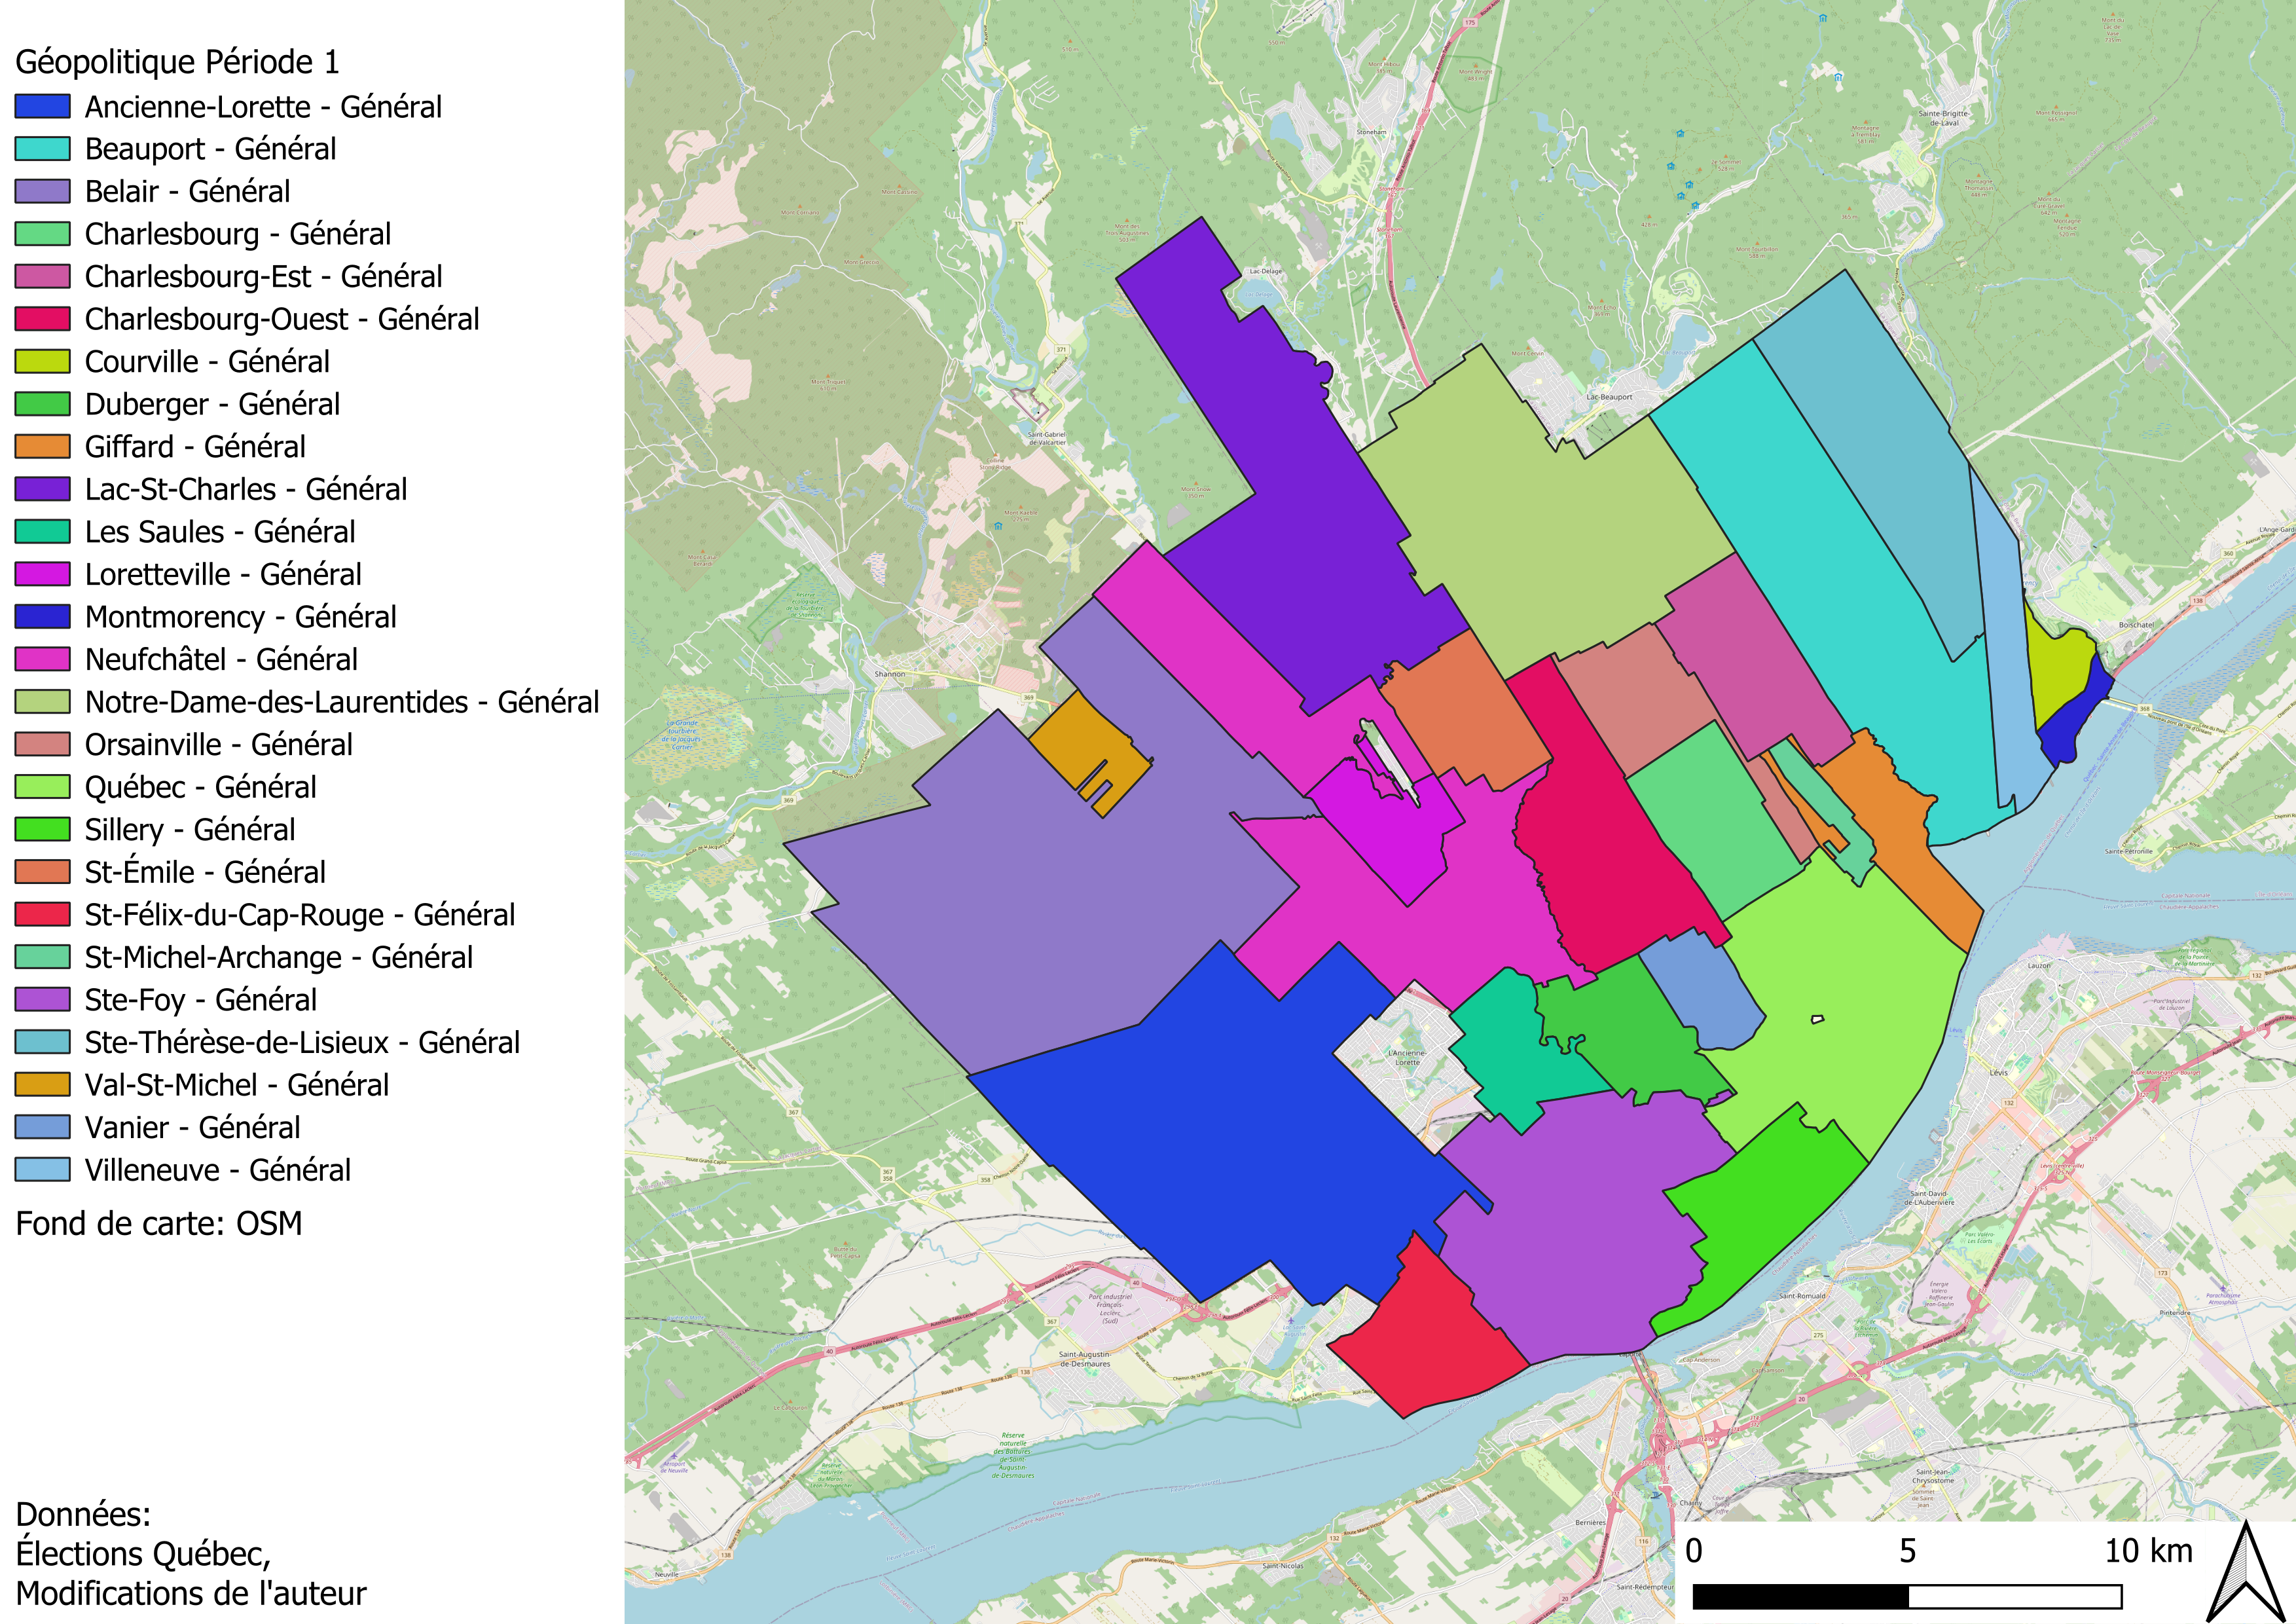
\includegraphics[width=15cm]{images/geopol-per-1}
    \caption{Découpage pour la période 1}\label{fig:ann-dec-per-1}
\end{figure}
\begin{figure}[H]
    \centering
    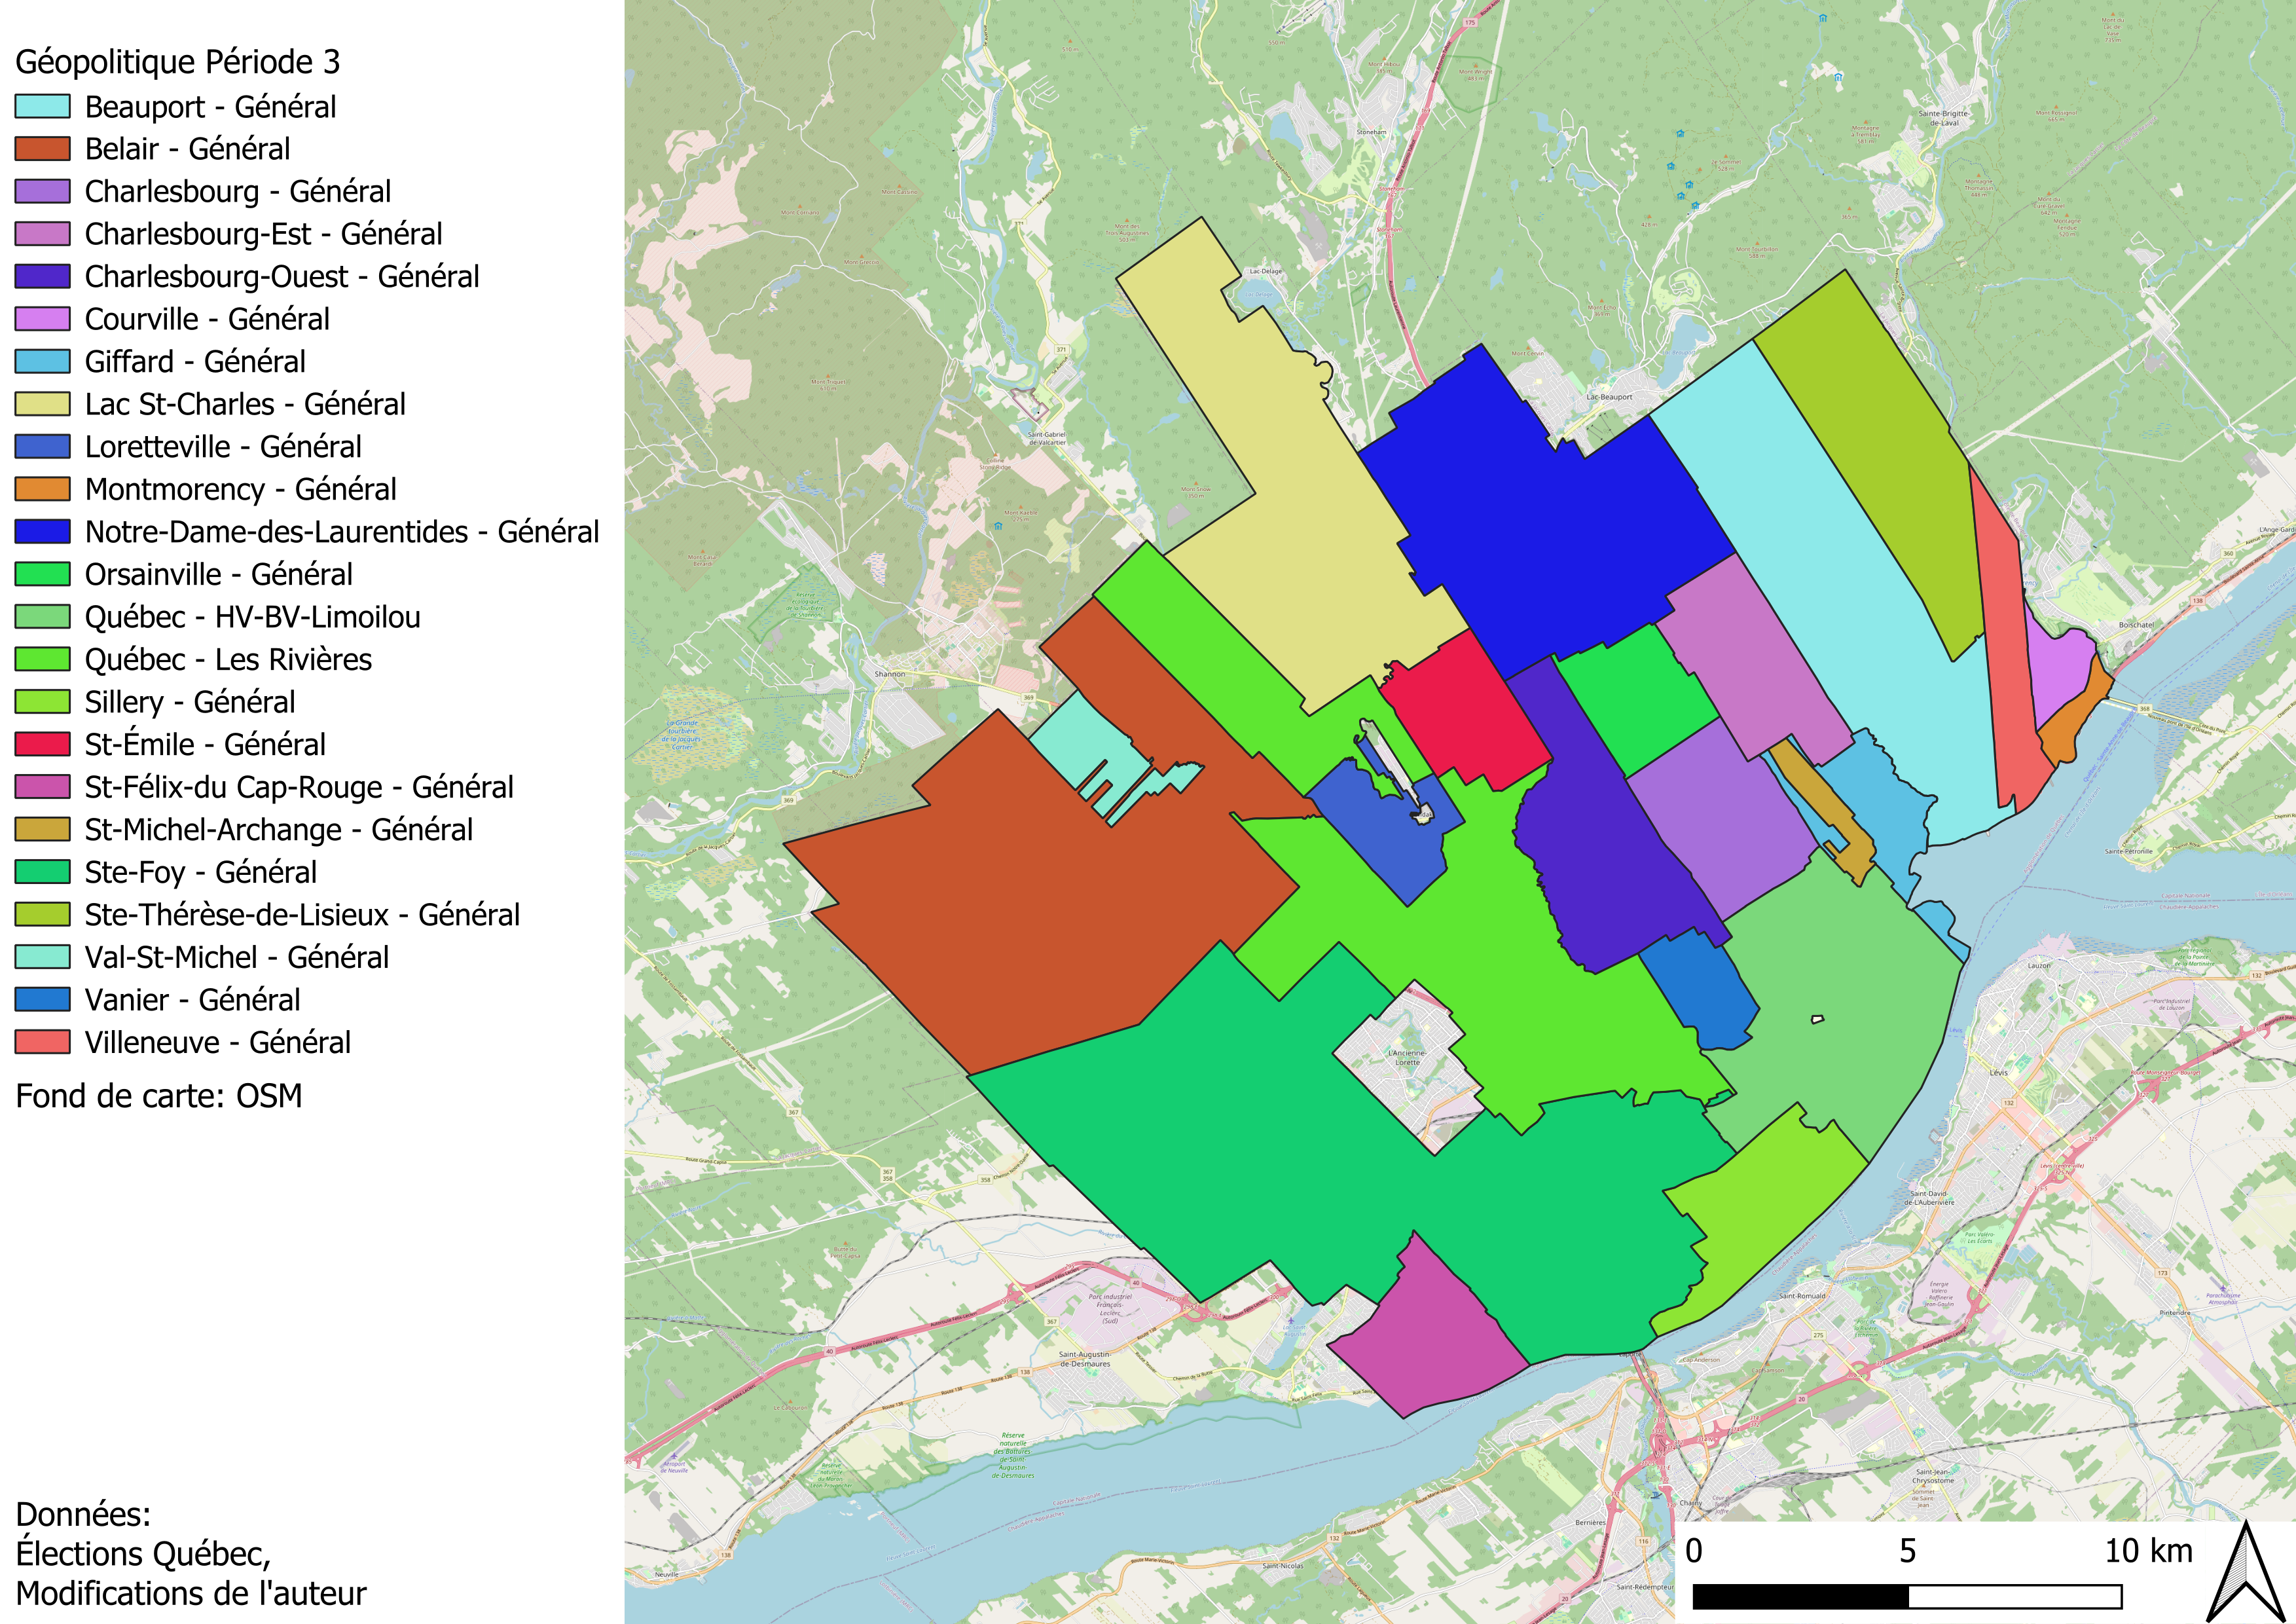
\includegraphics[width=15cm]{images/geopol-per-3}
    \caption{Découpage pour la période 3}\label{fig:ann-dec-per-3}
\end{figure}
\begin{figure}[H]
    \centering
    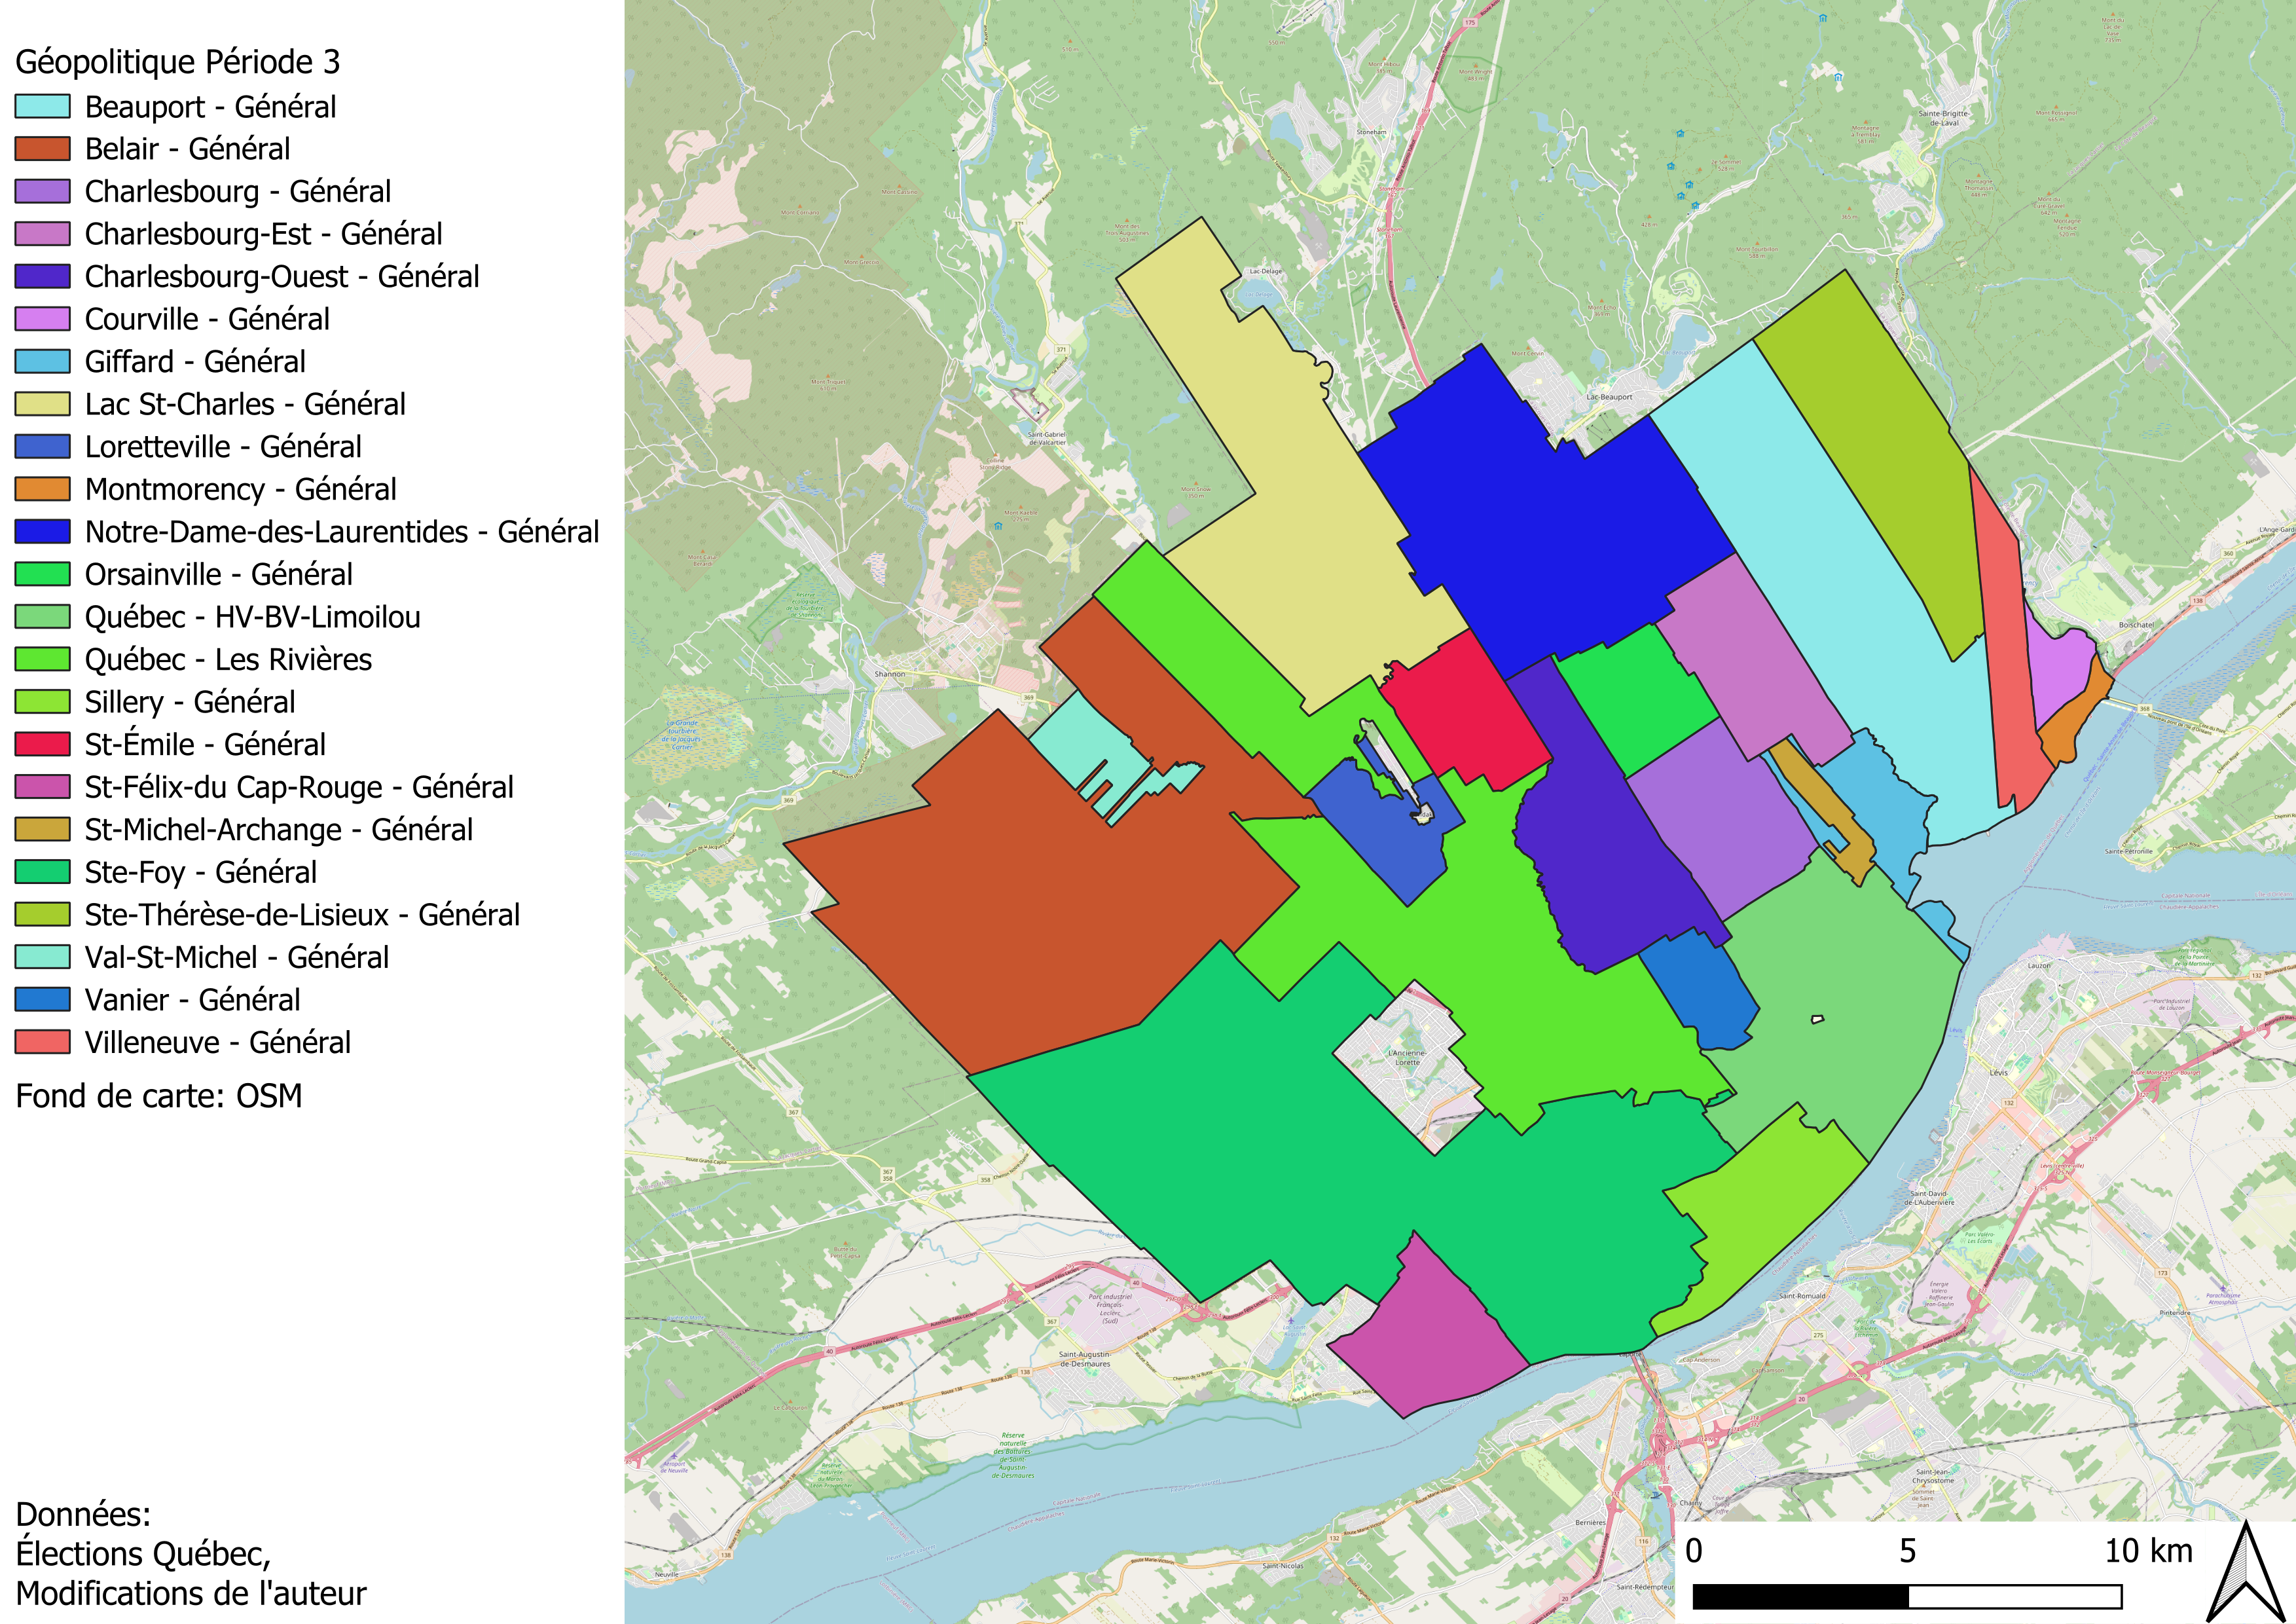
\includegraphics[width=15cm]{images/geopol-per-3}
    \caption{Découpage pour la période 4}\label{fig:ann-dec-per-4}
\end{figure}
\begin{figure}[H]
    \centering
    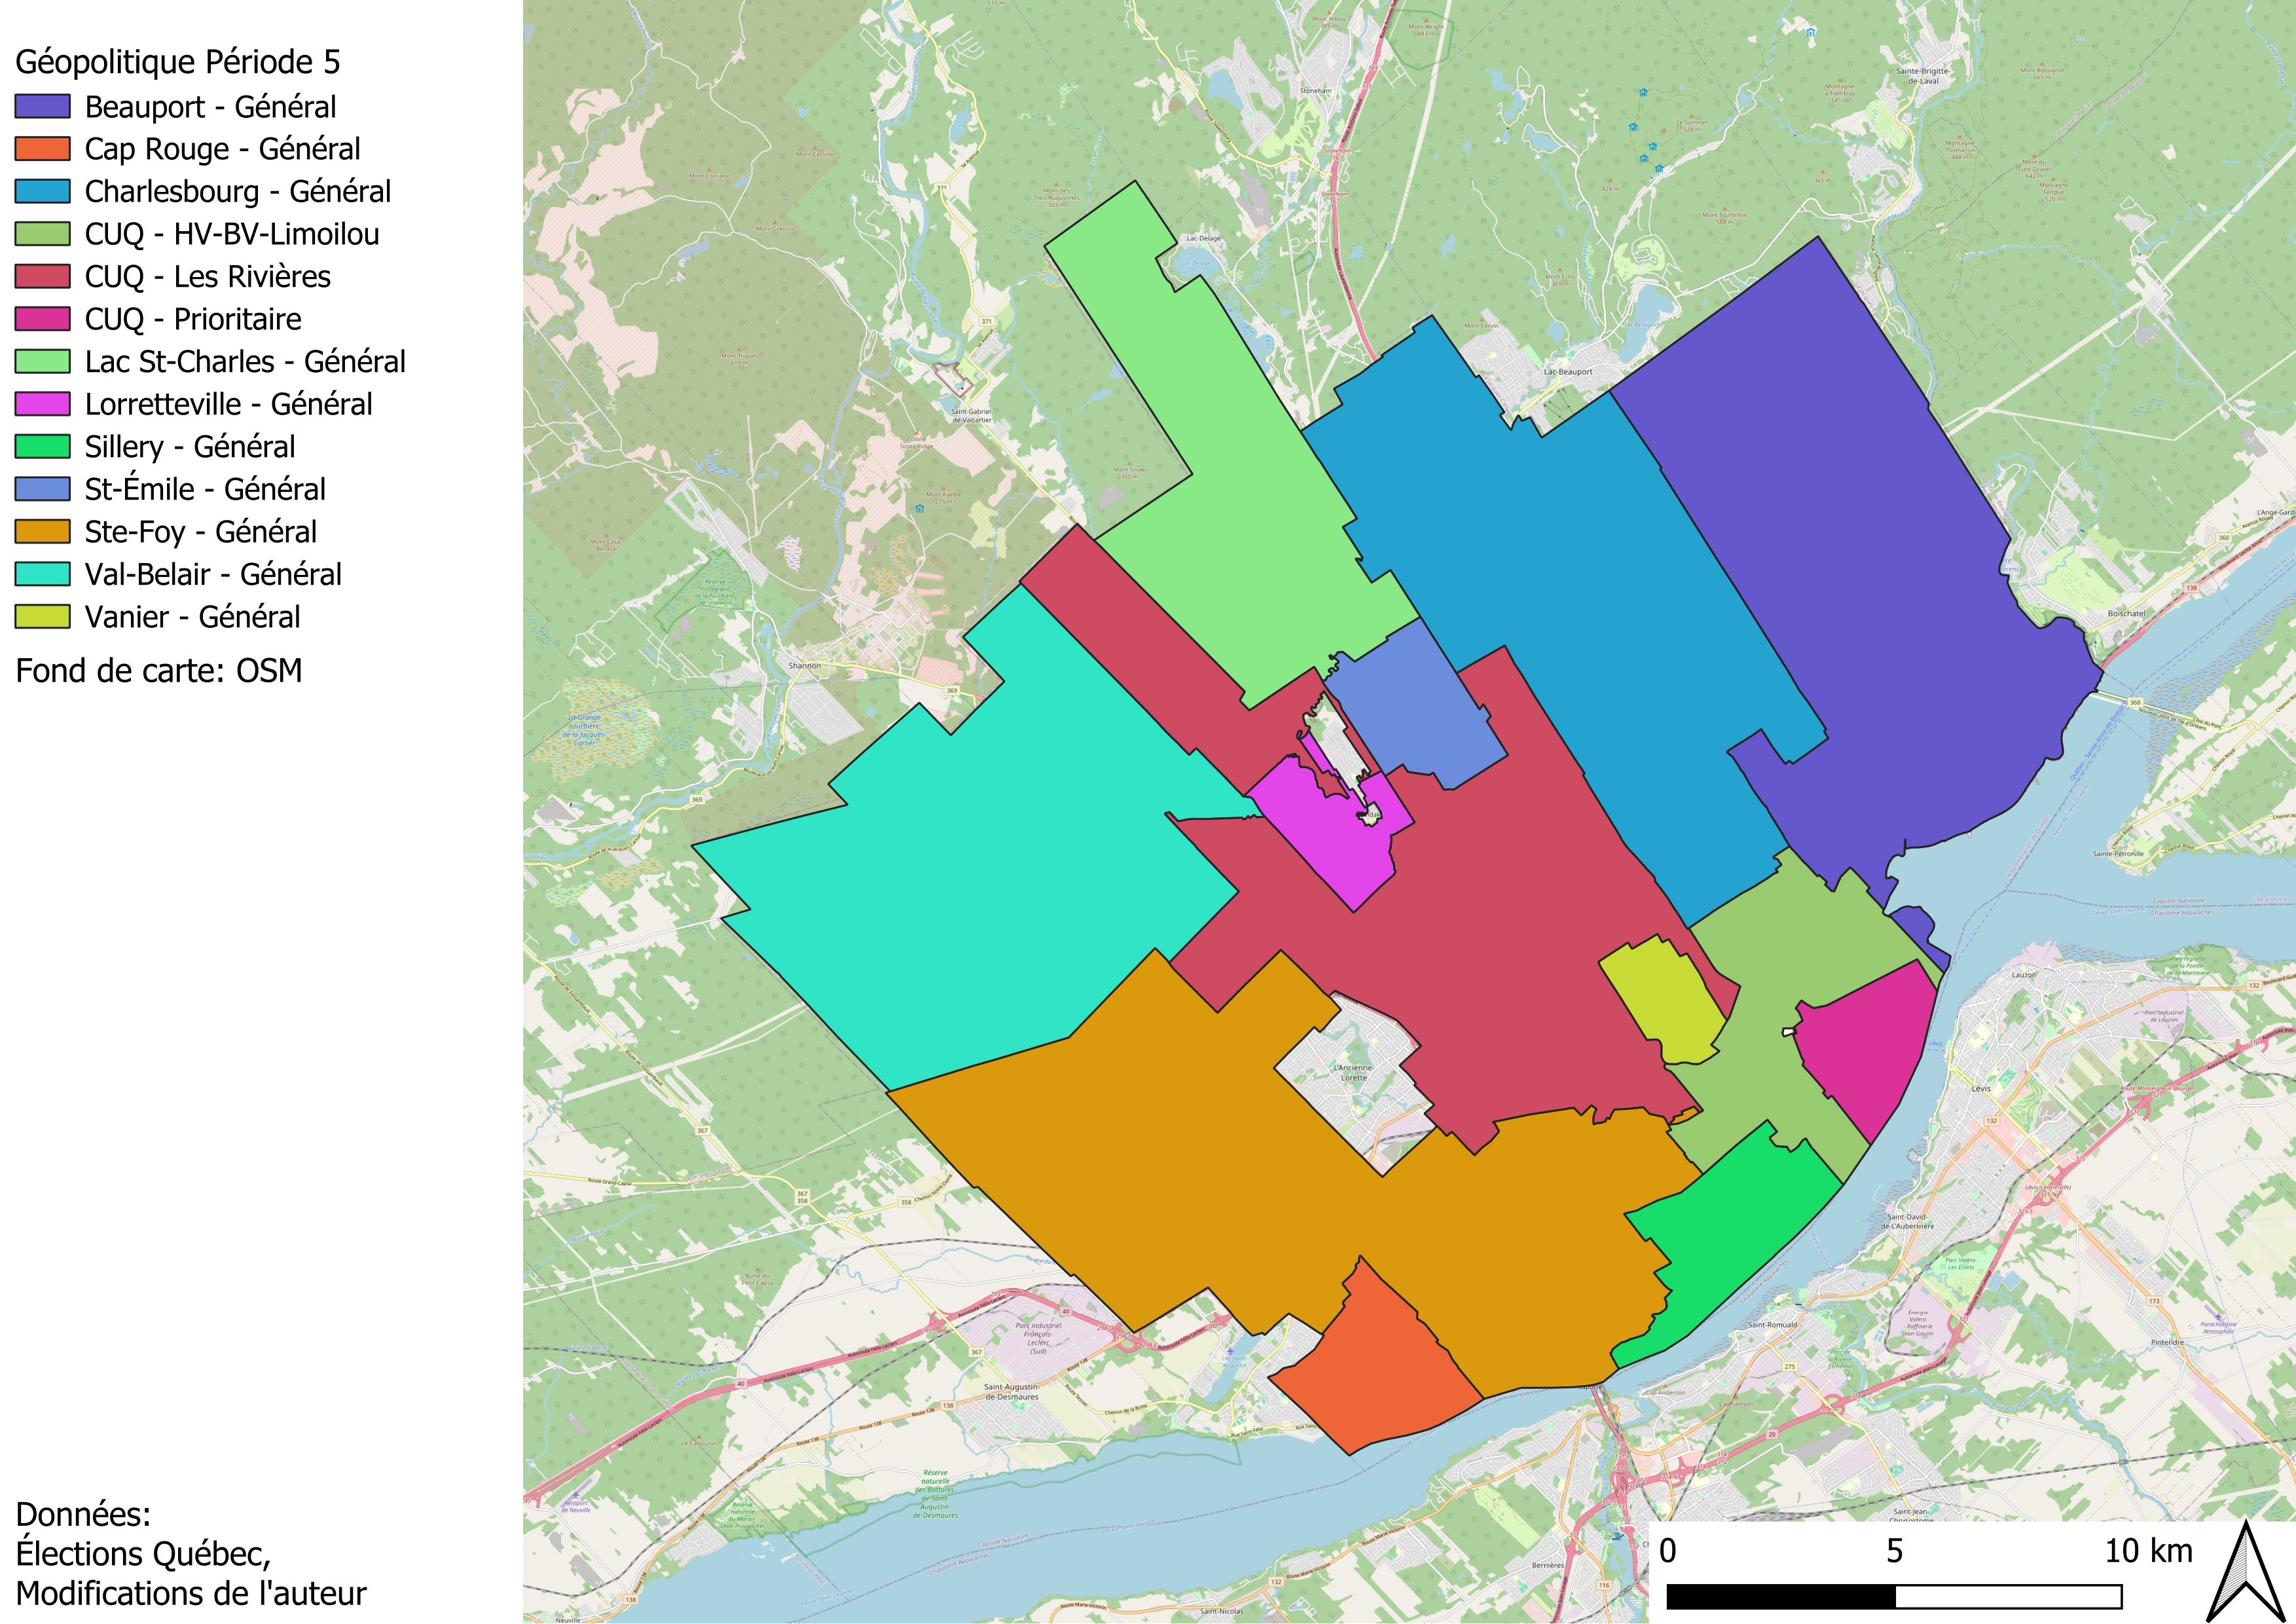
\includegraphics[width=15cm]{images/geopol-per-5}
    \caption{Découpage pour la période 5}\label{fig:ann-dec-per-5}
\end{figure}
\begin{figure}[H]
    \centering
    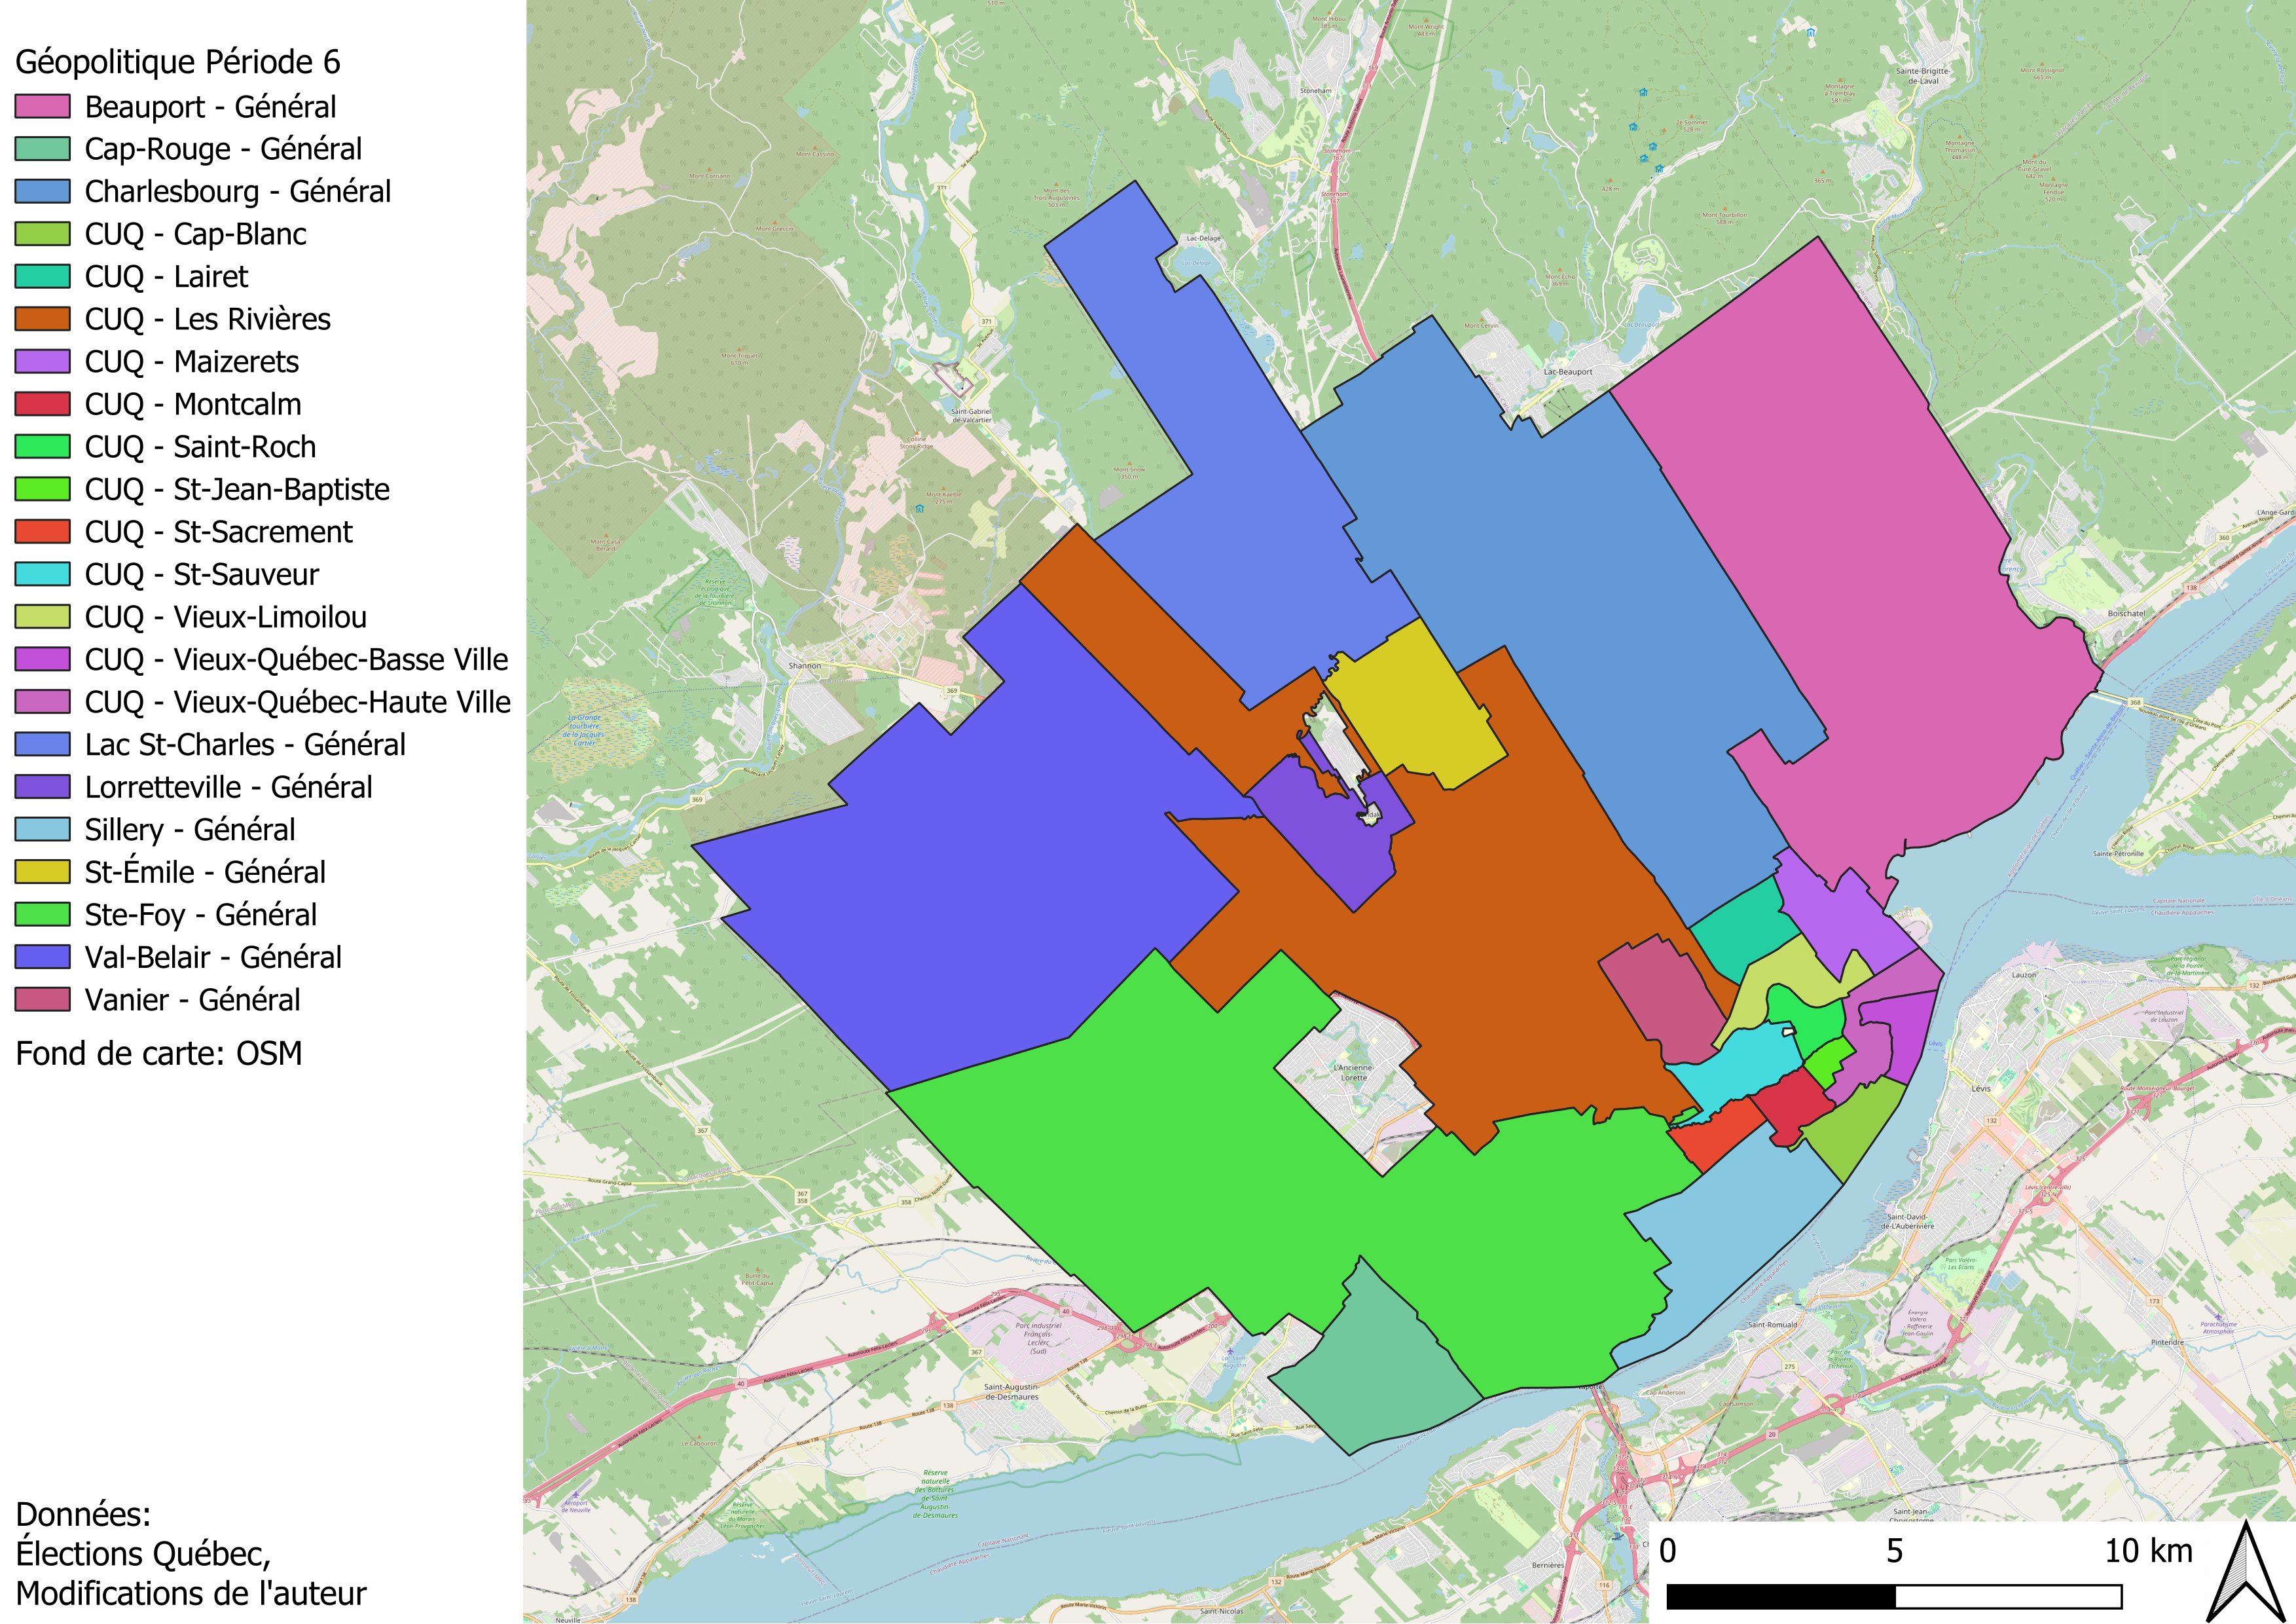
\includegraphics[width=15cm]{images/geopol-per-6}
    \caption{Découpage pour la période 6}\label{fig:ann-dec-per-6}
\end{figure}
\begin{figure}[H]
    \centering
    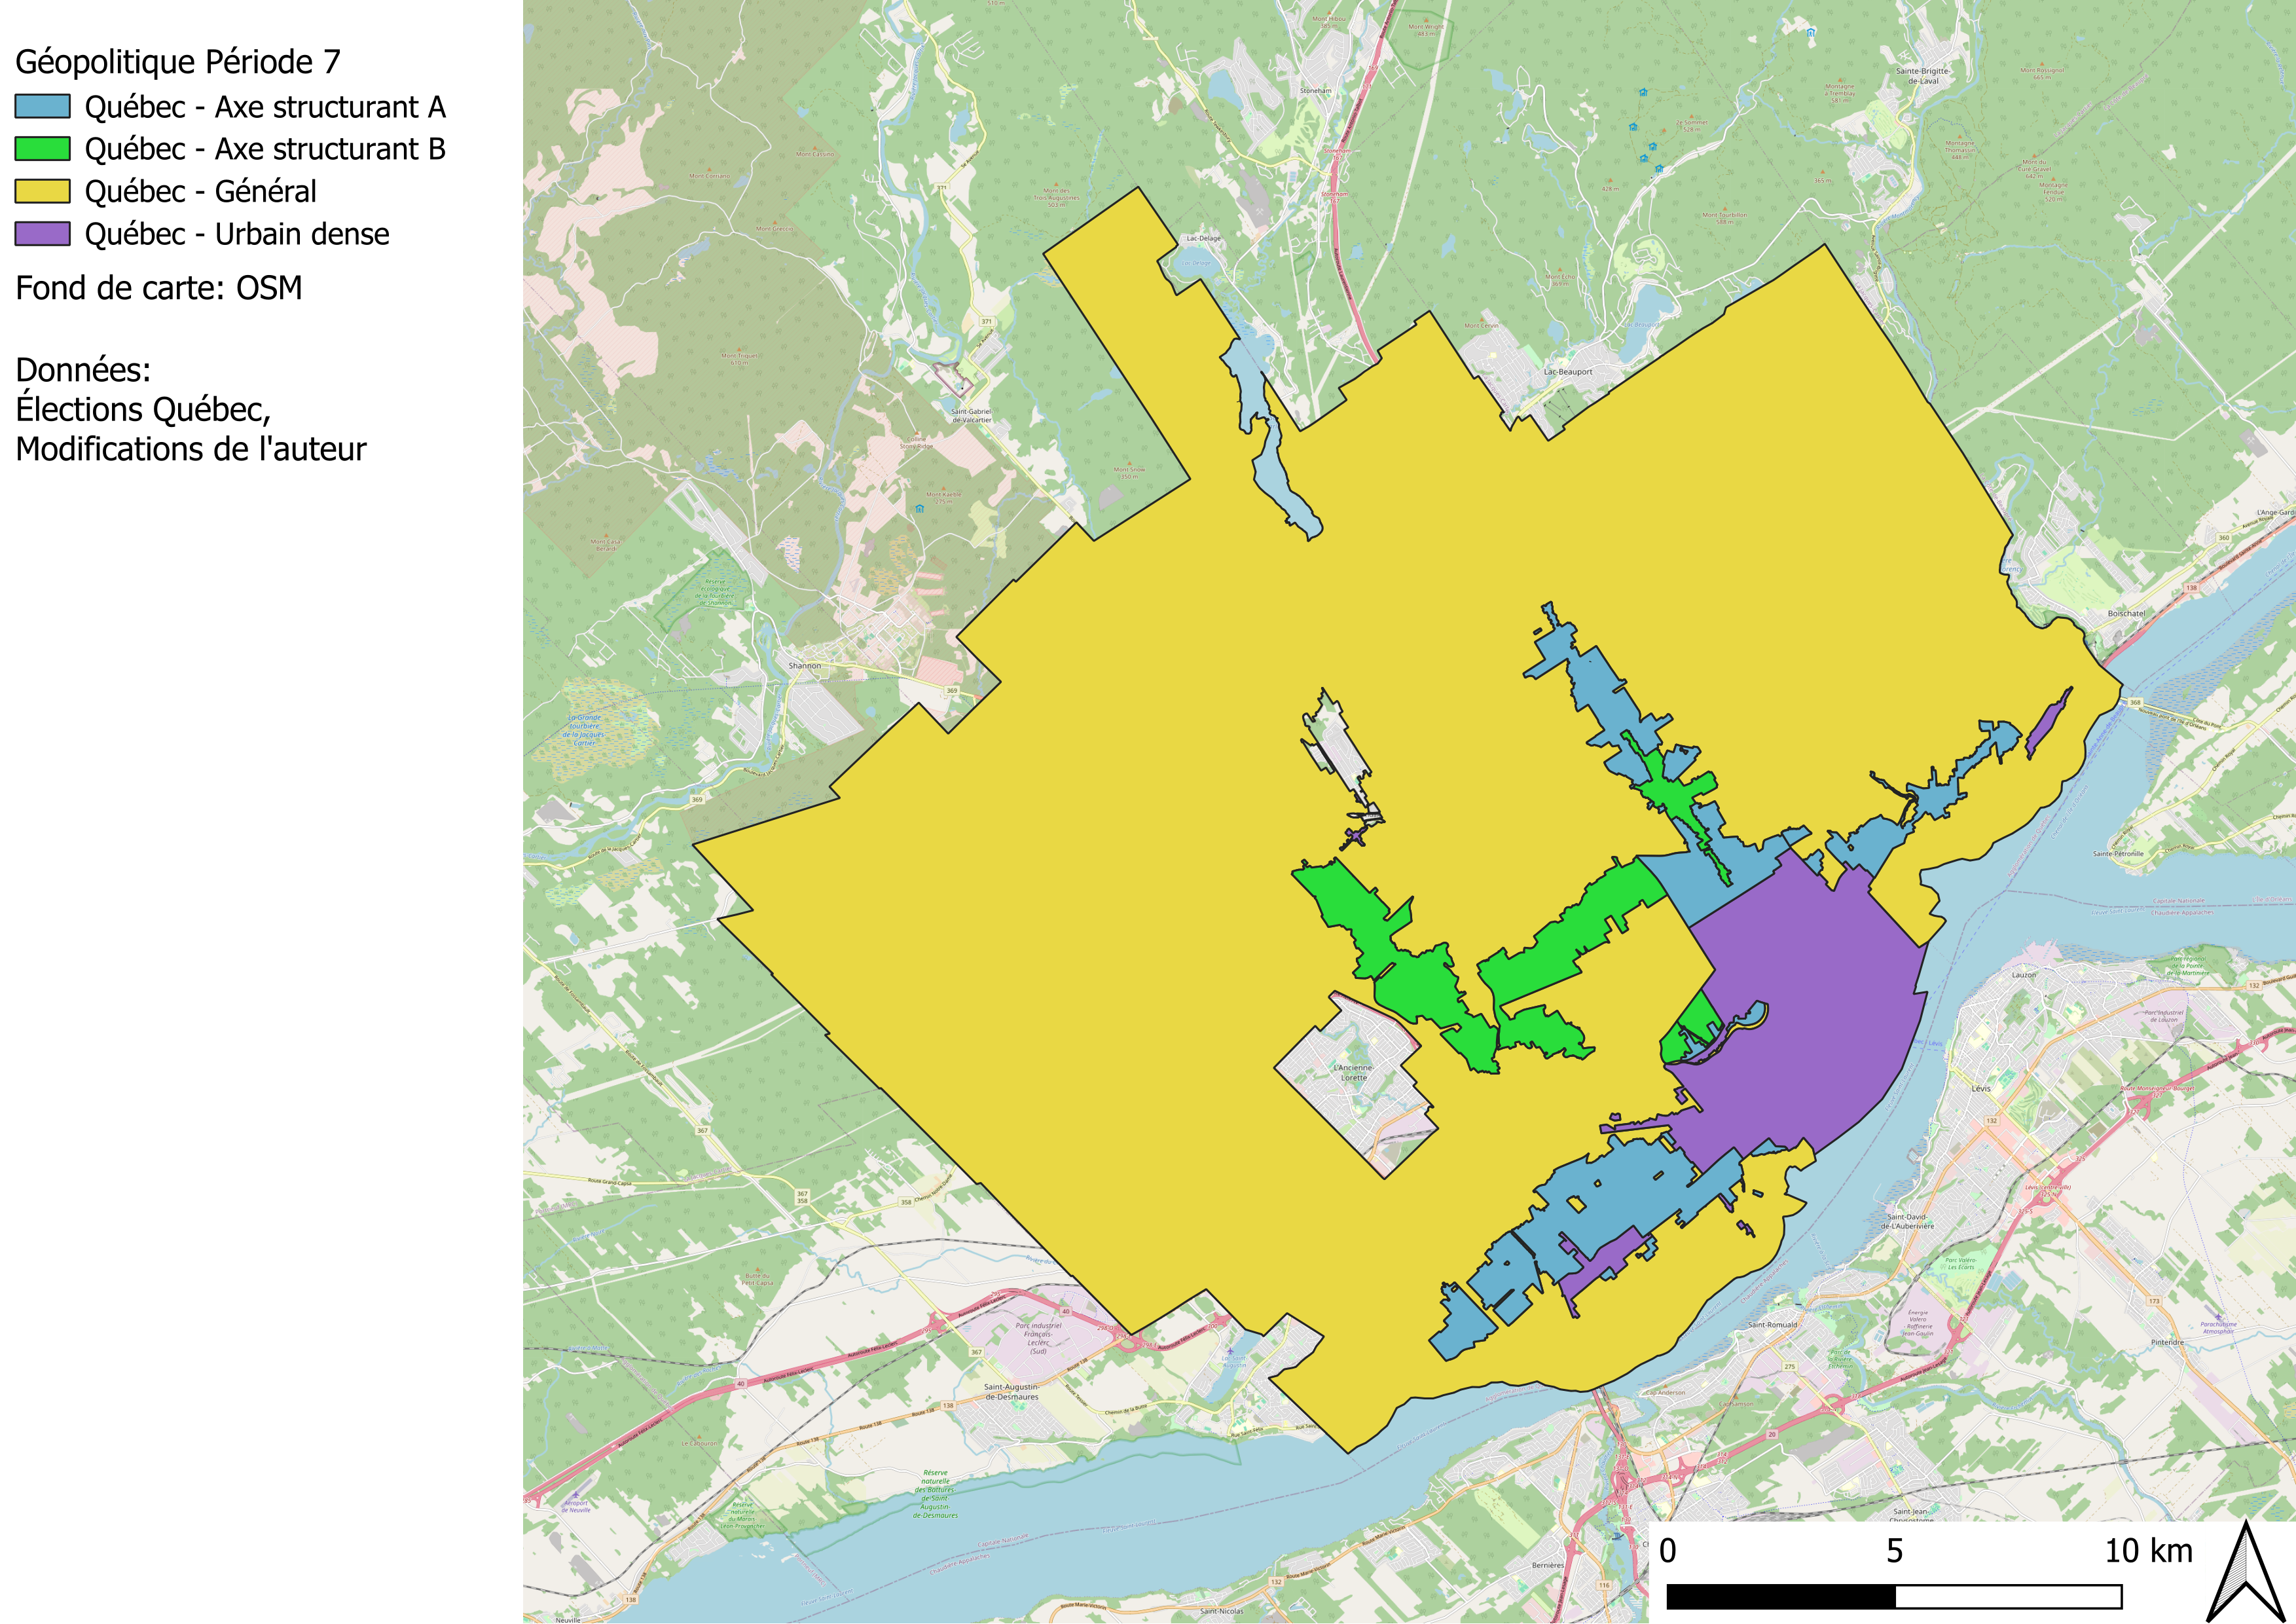
\includegraphics[width=15cm]{images/geopol-per-7}
    \caption{Découpage pour la période 7}\label{fig:ann-dec-per-7}
\end{figure}